%!TEX program = xelatex
\documentclass[cn,hazy,pku,12pt,normal,math=newtx,cite=super]{elegantnote}
\title{紫外可见光吸收光谱仪的搭建与\\量子一维势阱方程的检验}

\author{刘松瑞 \quad 2100011819 \\ 组号:24 \quad 组内编号:5 \quad 合作者:万乘}
\institute{化学与分子工程学院}

\expdate{\zhdate{2023/9/28}}
\temperature{20.1 \si{^{\circ}C}}
\pressure{101.38 \si{kPa}}

\usepackage{array}
\usepackage{subfigure}
\usepackage[fontset=windows]{ctex}
\usepackage{graphicx}
\usepackage{float}
\usepackage{caption}
\usepackage{multirow}
%\usepackage{subfig}
%\usepackage{float}
\begin{document}

\maketitle

\keywords{紫外-可见光谱\quad一维势阱模型\quad花菁染料\quad TDDFT}

\abstracts{
    本实验通过搭建紫外可见光谱仪,测定多种分子的最大吸收波长与紫外可见吸收光谱。
    并讨论光源、浓度等因素对吸收光谱的影响。
    最后使用一维势阱模型和量子化学计算的方法对实验的结果进行比较,并研究大共轭分子的跃迁波长规律
    以及与一维势阱模型之间的联系。
}

\newpage


\section{引言}

\subsection{实验目的、原理}

实验目的、原理详见预习报告图 ~\ref{1} 。

\begin{figure}[htbp]
    \centering
    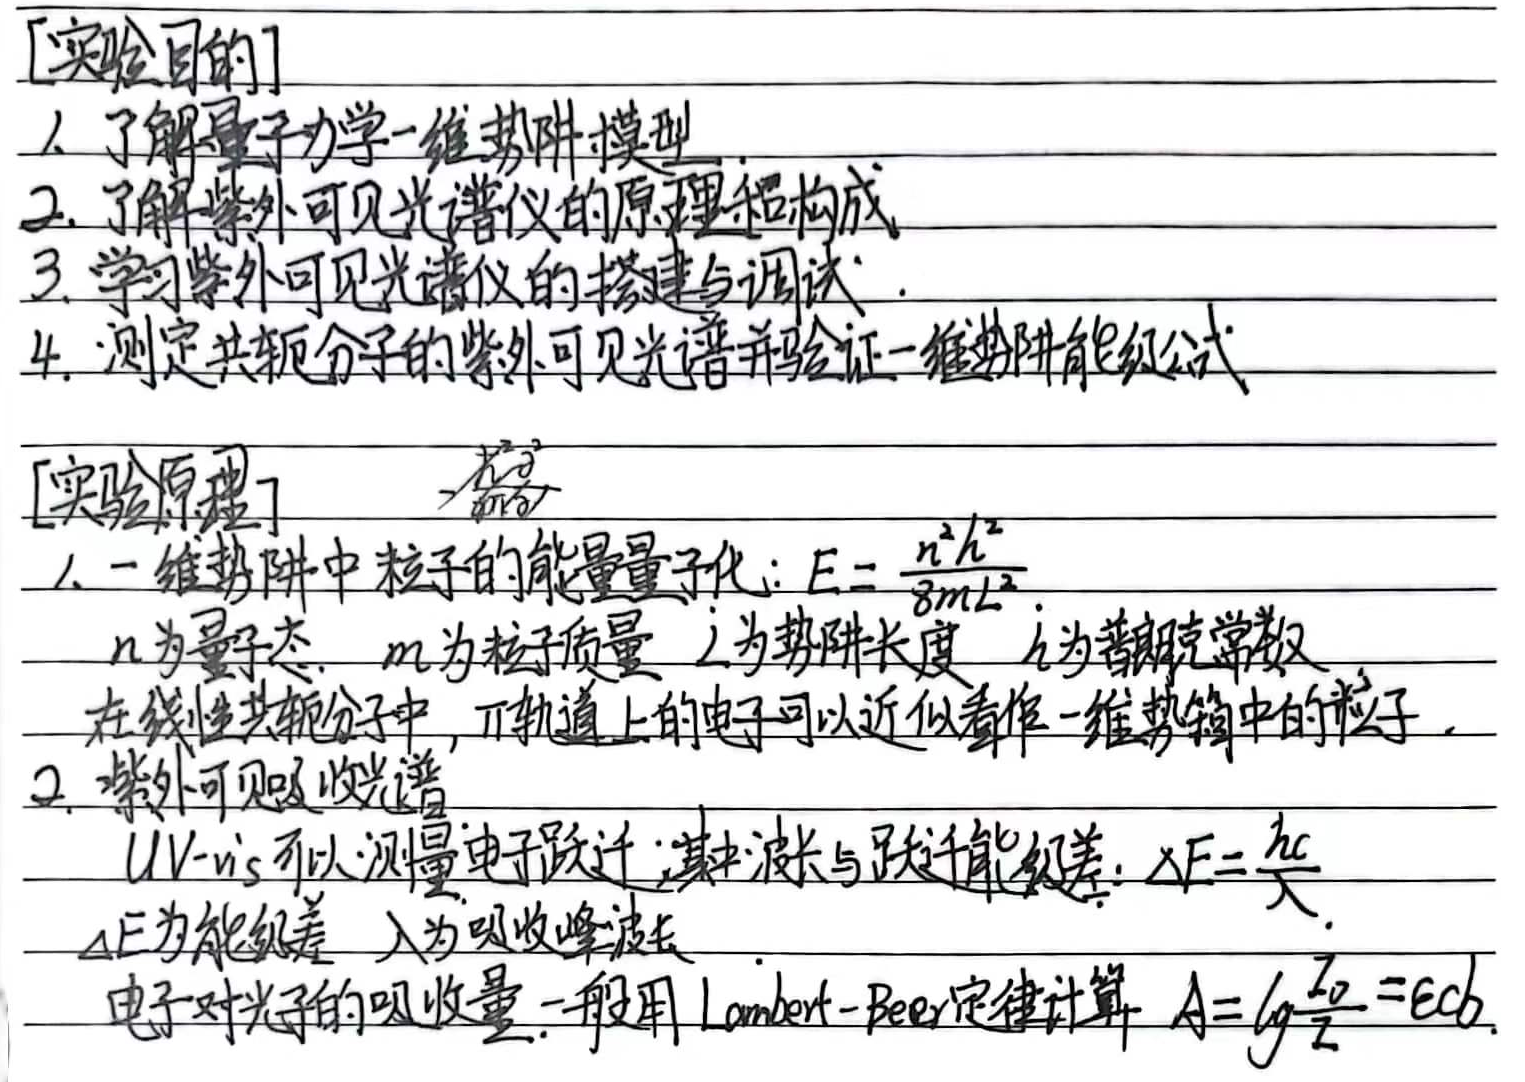
\includegraphics[width = .88\textwidth]{image/yxbg_1.png}
    \caption{实验的目的、原理}\label{1}
\end{figure}

\subsection{实验方法}

搭建紫外可见光谱仪,并测定一系列溶液的吸光度。通过紫外可见光谱仪的数据验证量子一维势阱的结论。

\section{实验部分}

\subsection{实验步骤}

实验步骤详见预习报告图~\ref{a} 与图~\ref{4} 。

\begin{figure}[htbp]
    \centering
    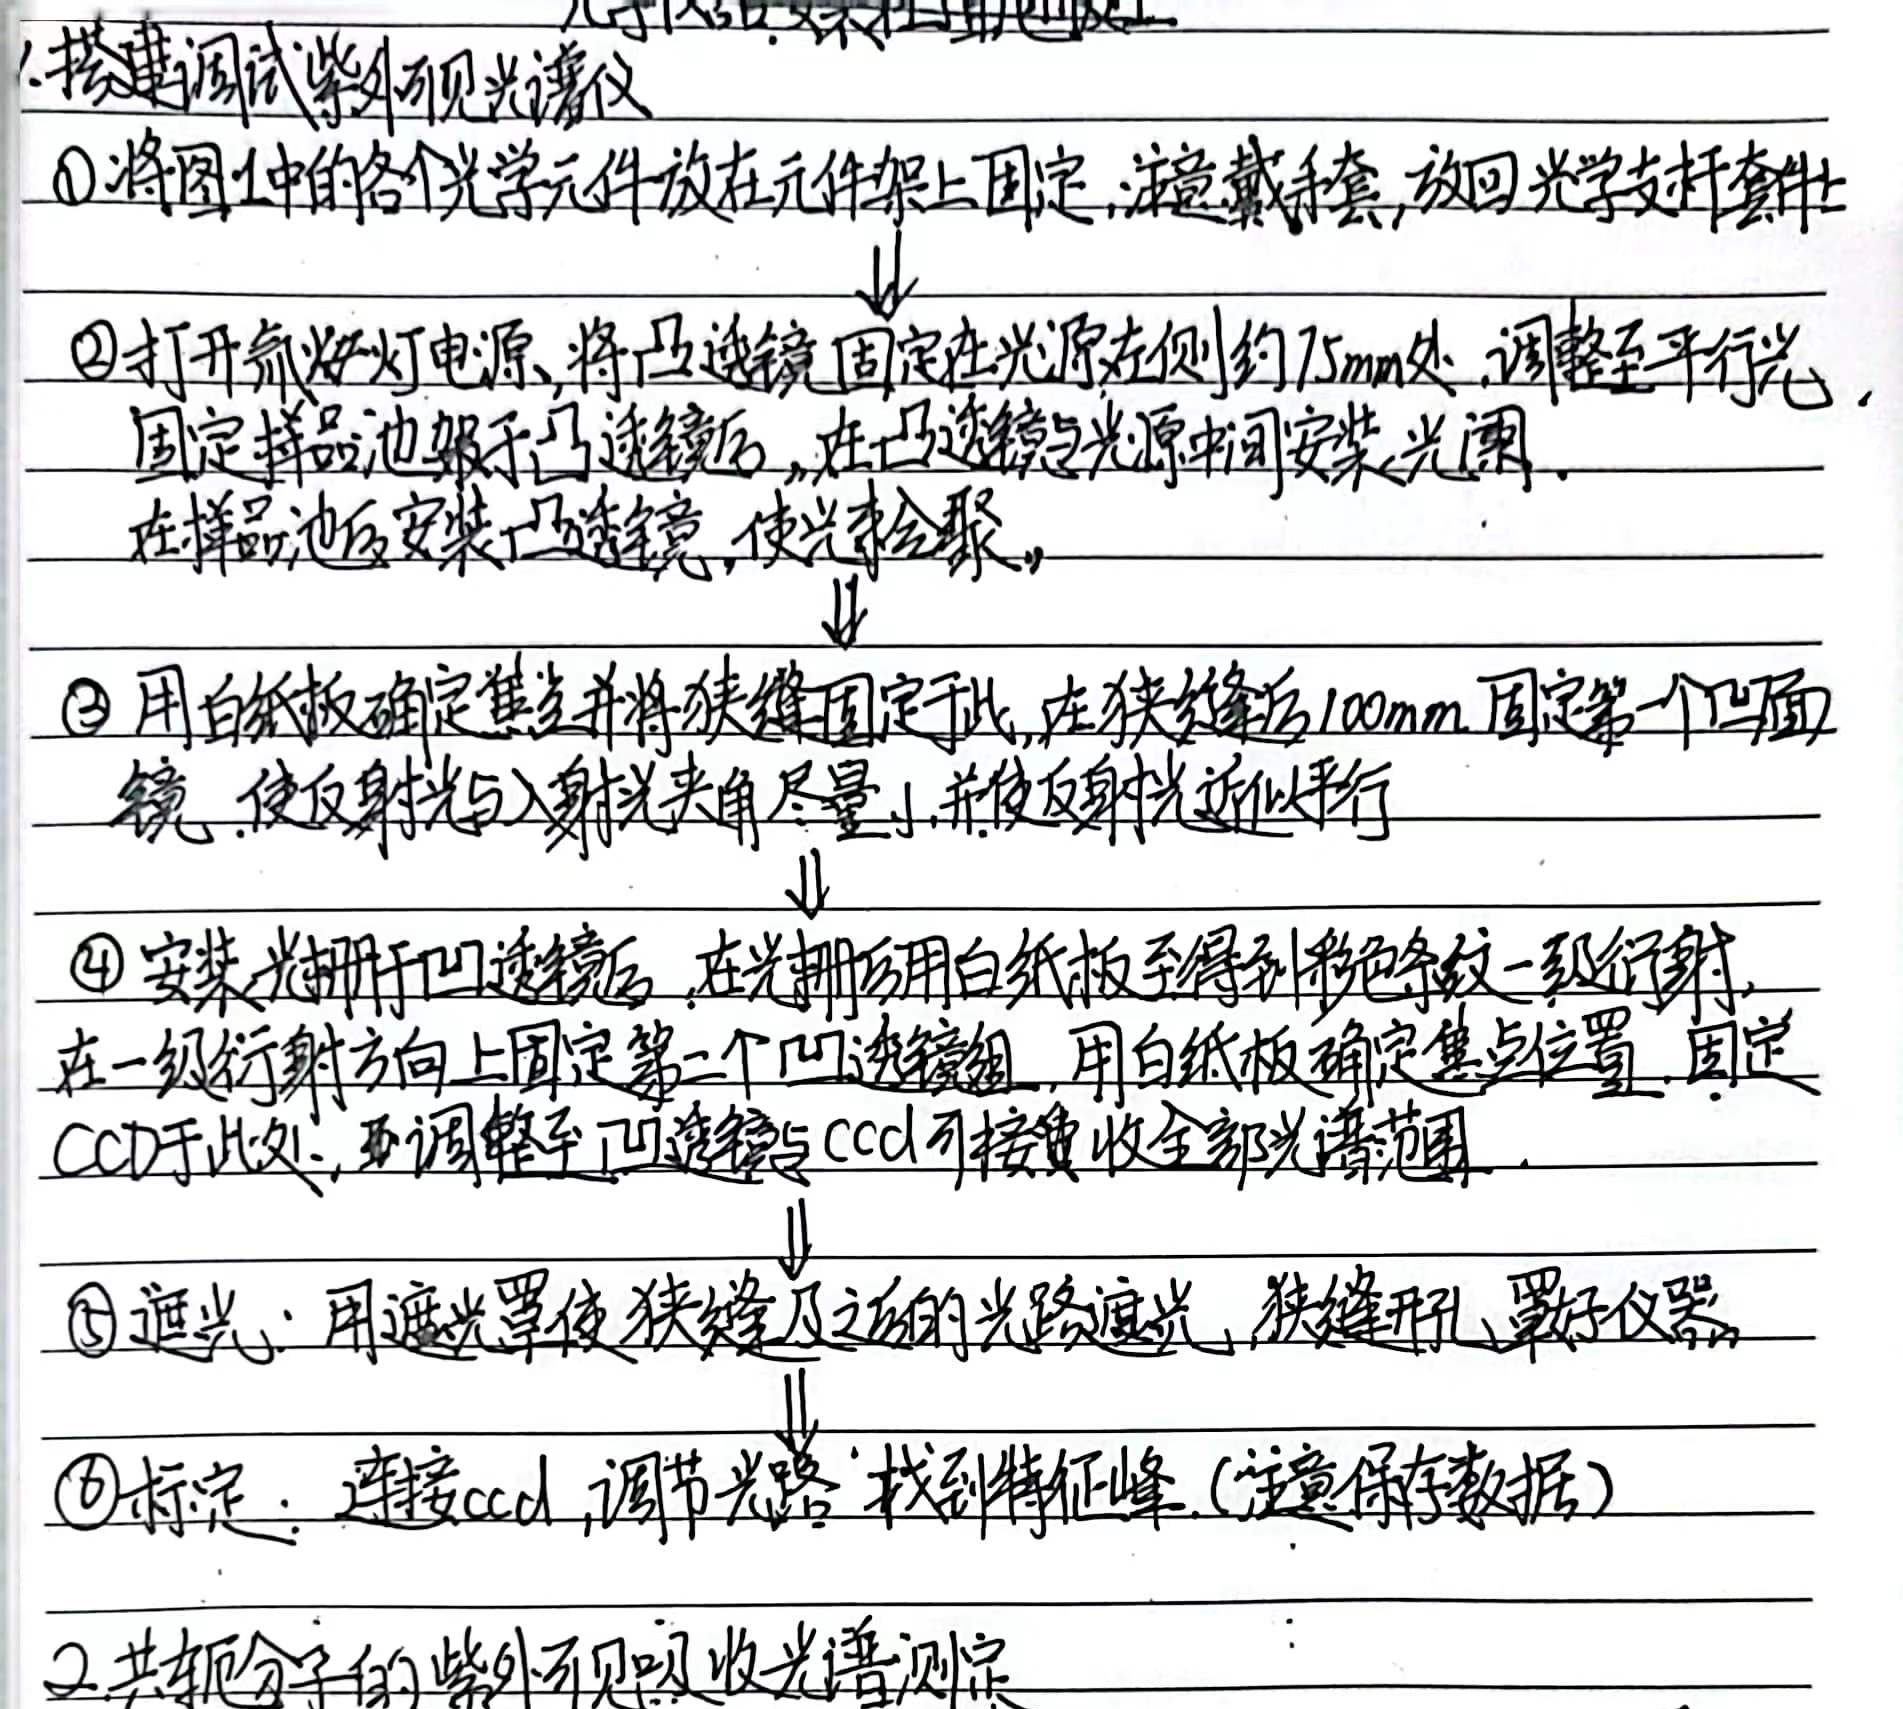
\includegraphics[width = .88\textwidth]{image/yxbg_2.5.png}
    \caption{实验步骤}\label{a}
\end{figure}

\begin{figure}[htbp]
    \centering
    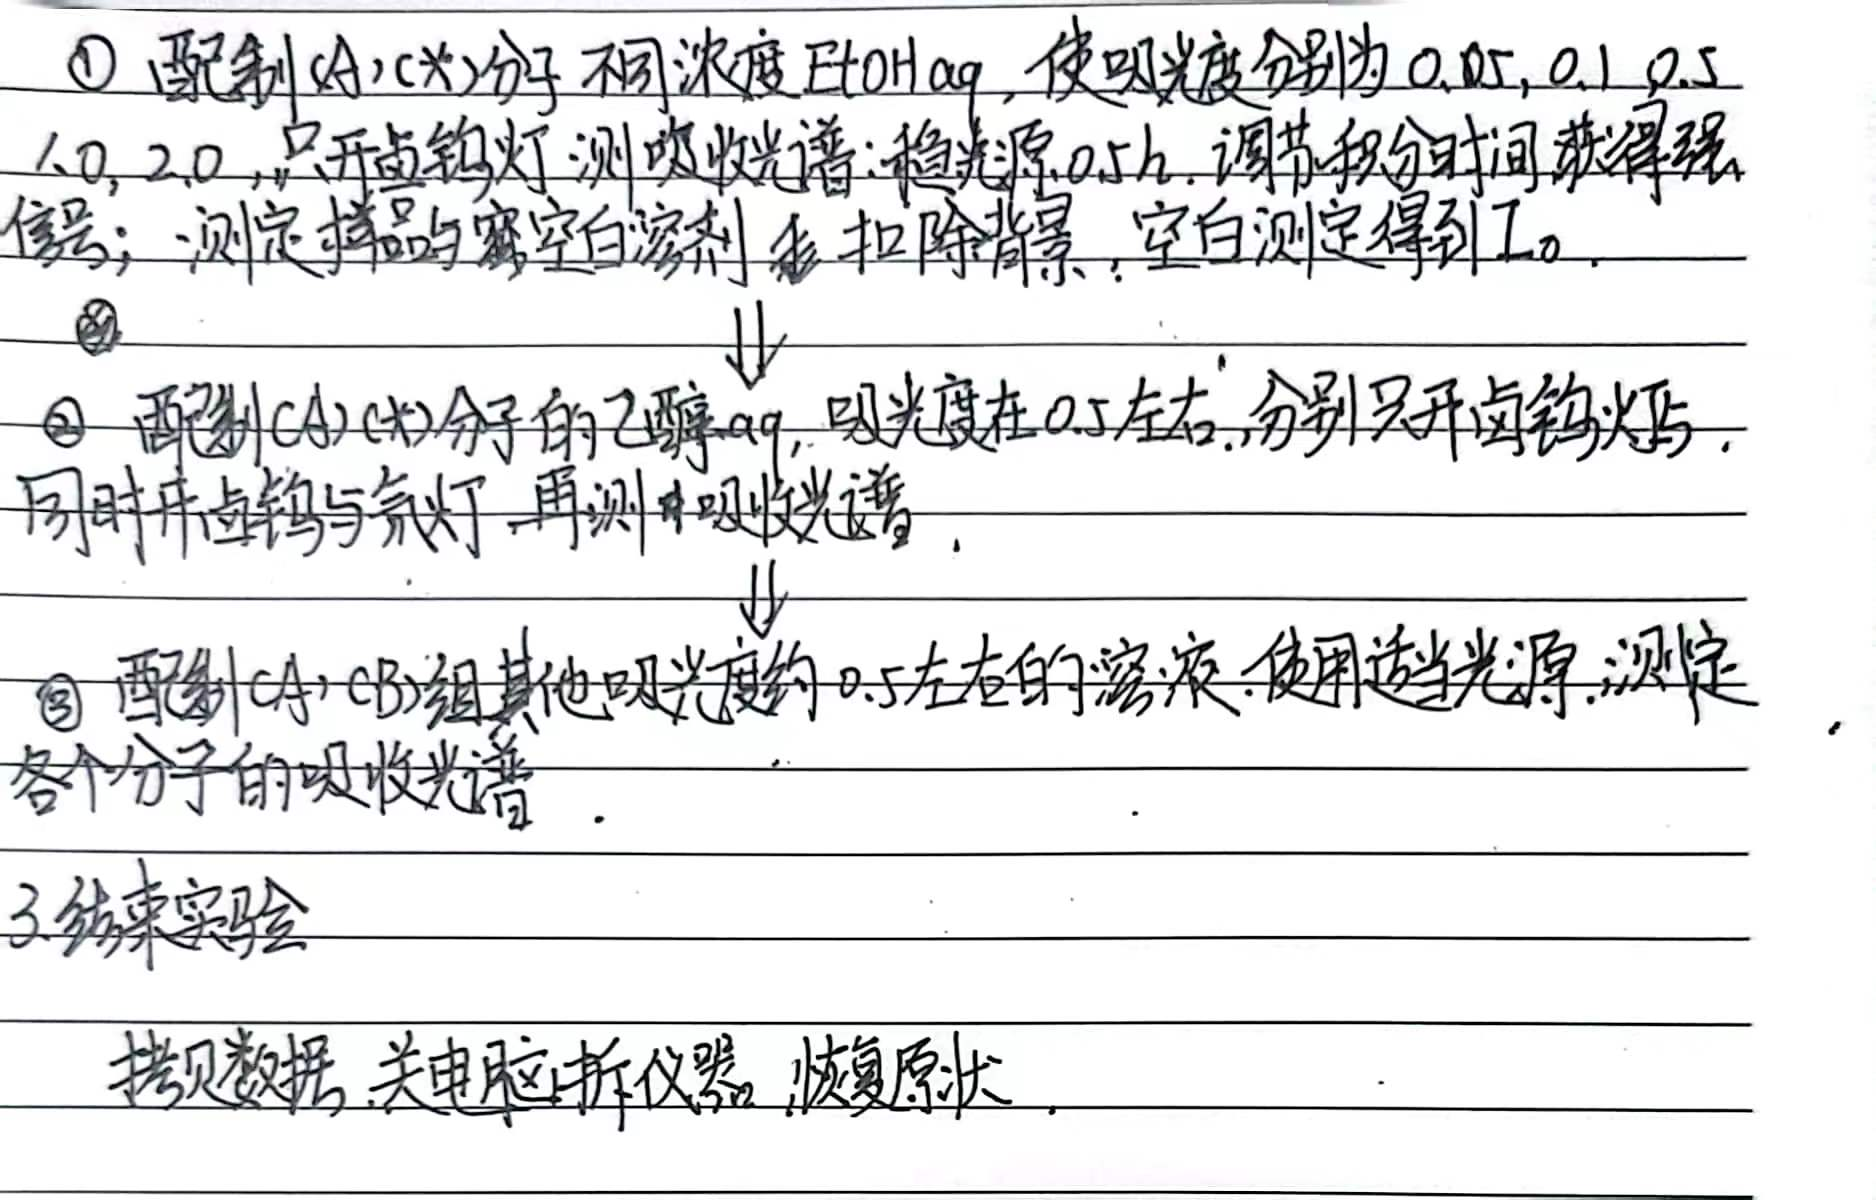
\includegraphics[width = .88\textwidth]{image/yxbg_3.jpg}
    \caption{实验步骤}\label{4}
\end{figure}

\subsection{仪器与药品}

\begin{enumerate} %有序列表
    \item 试剂 \\ 无水乙醇,标准浓度的六种染料(如图~\ref{2} )的乙醇溶液。
    \item 光谱仪部件 \\ 光源(氘灯,钨灯,汞灯),光阑,平凸透镜,样品池架,狭缝,凹面镜,光栅,CCD
    检测器,光学平台(面包板),光学元件架,光学支杆套件,遮光器材,安装工具。
\end{enumerate}


\begin{figure}[htbp]
    \centering
    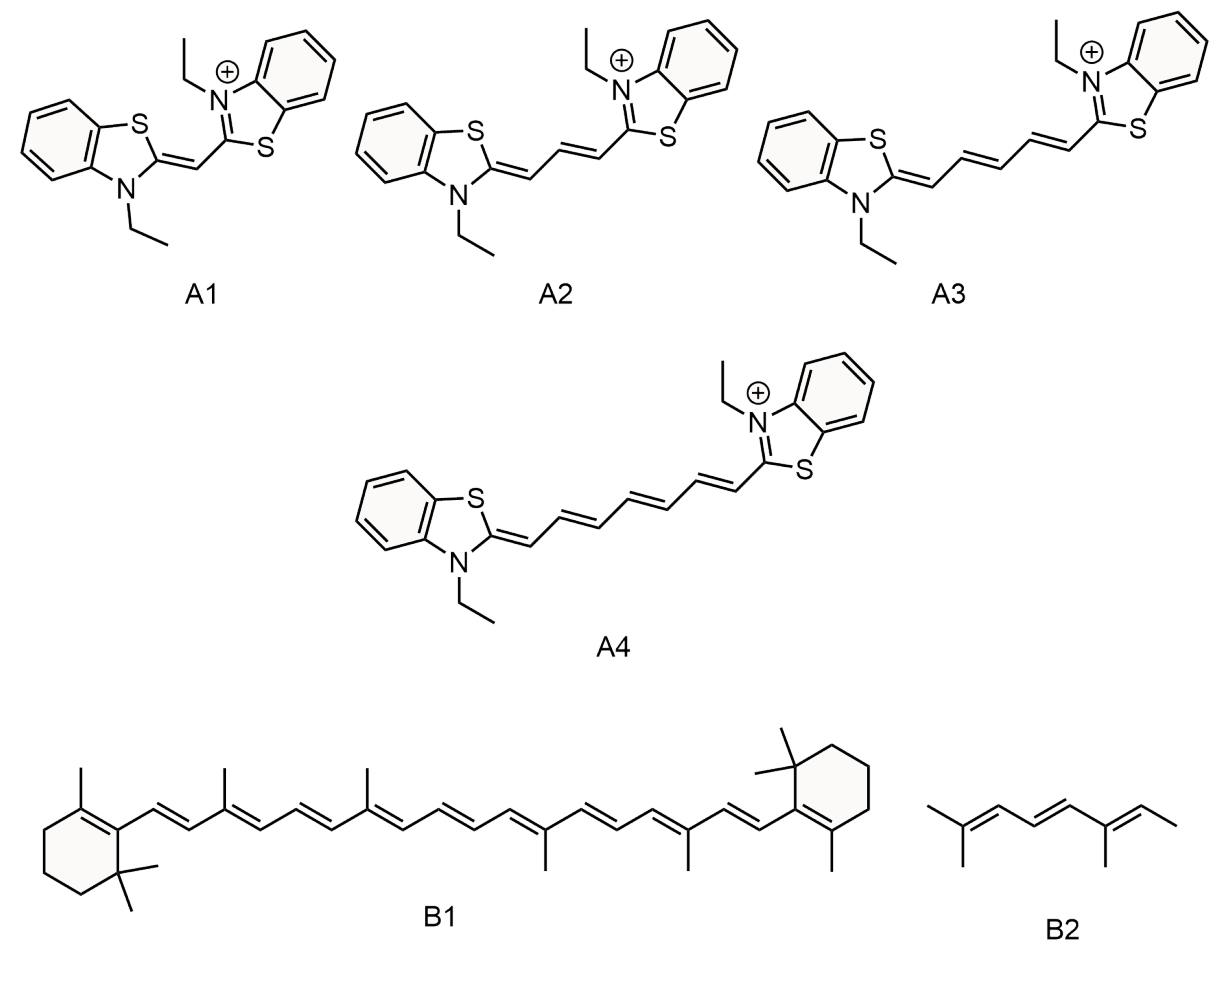
\includegraphics[width = .60\textwidth]{image/drugs.png}
    \caption{待测样品分子}\label{2}
\end{figure}

\section{实验现象与数据处理}

\subsection{光谱仪的标定}

按照实验步骤进行紫外可见光谱仪器的搭建,打开氘灯,调整 CCD 的位置至出现三个明显的
特征峰,并与标准图谱~\ref{5-} 比对,如下图~\ref{5--} 所示。

将三个特征峰与标准谱图进行比对如表~\ref{6} ,线性拟合如图~\ref{7} ,可以
得到 $\lambda$ 与  $ {\rm Pixel} $ 线性关系为:
\begin{equation}\label{nihe}
    \lambda = (347.88694 \pm  1.14631) + (0.13069 \pm  0.00063) * {\rm Pixel} \quad R^2=0.99996
\end{equation}

实验所用的 CCD 像素点范围为 1 - 3648,则有可测量的光谱范围为 348.07 - 824.60 nm。
考虑到两侧的信噪比较高,实际测量范围为350 - 750 nm,可以准确测定偏向于红外光区的分子。



\begin{figure}[htbp]
    \centering
    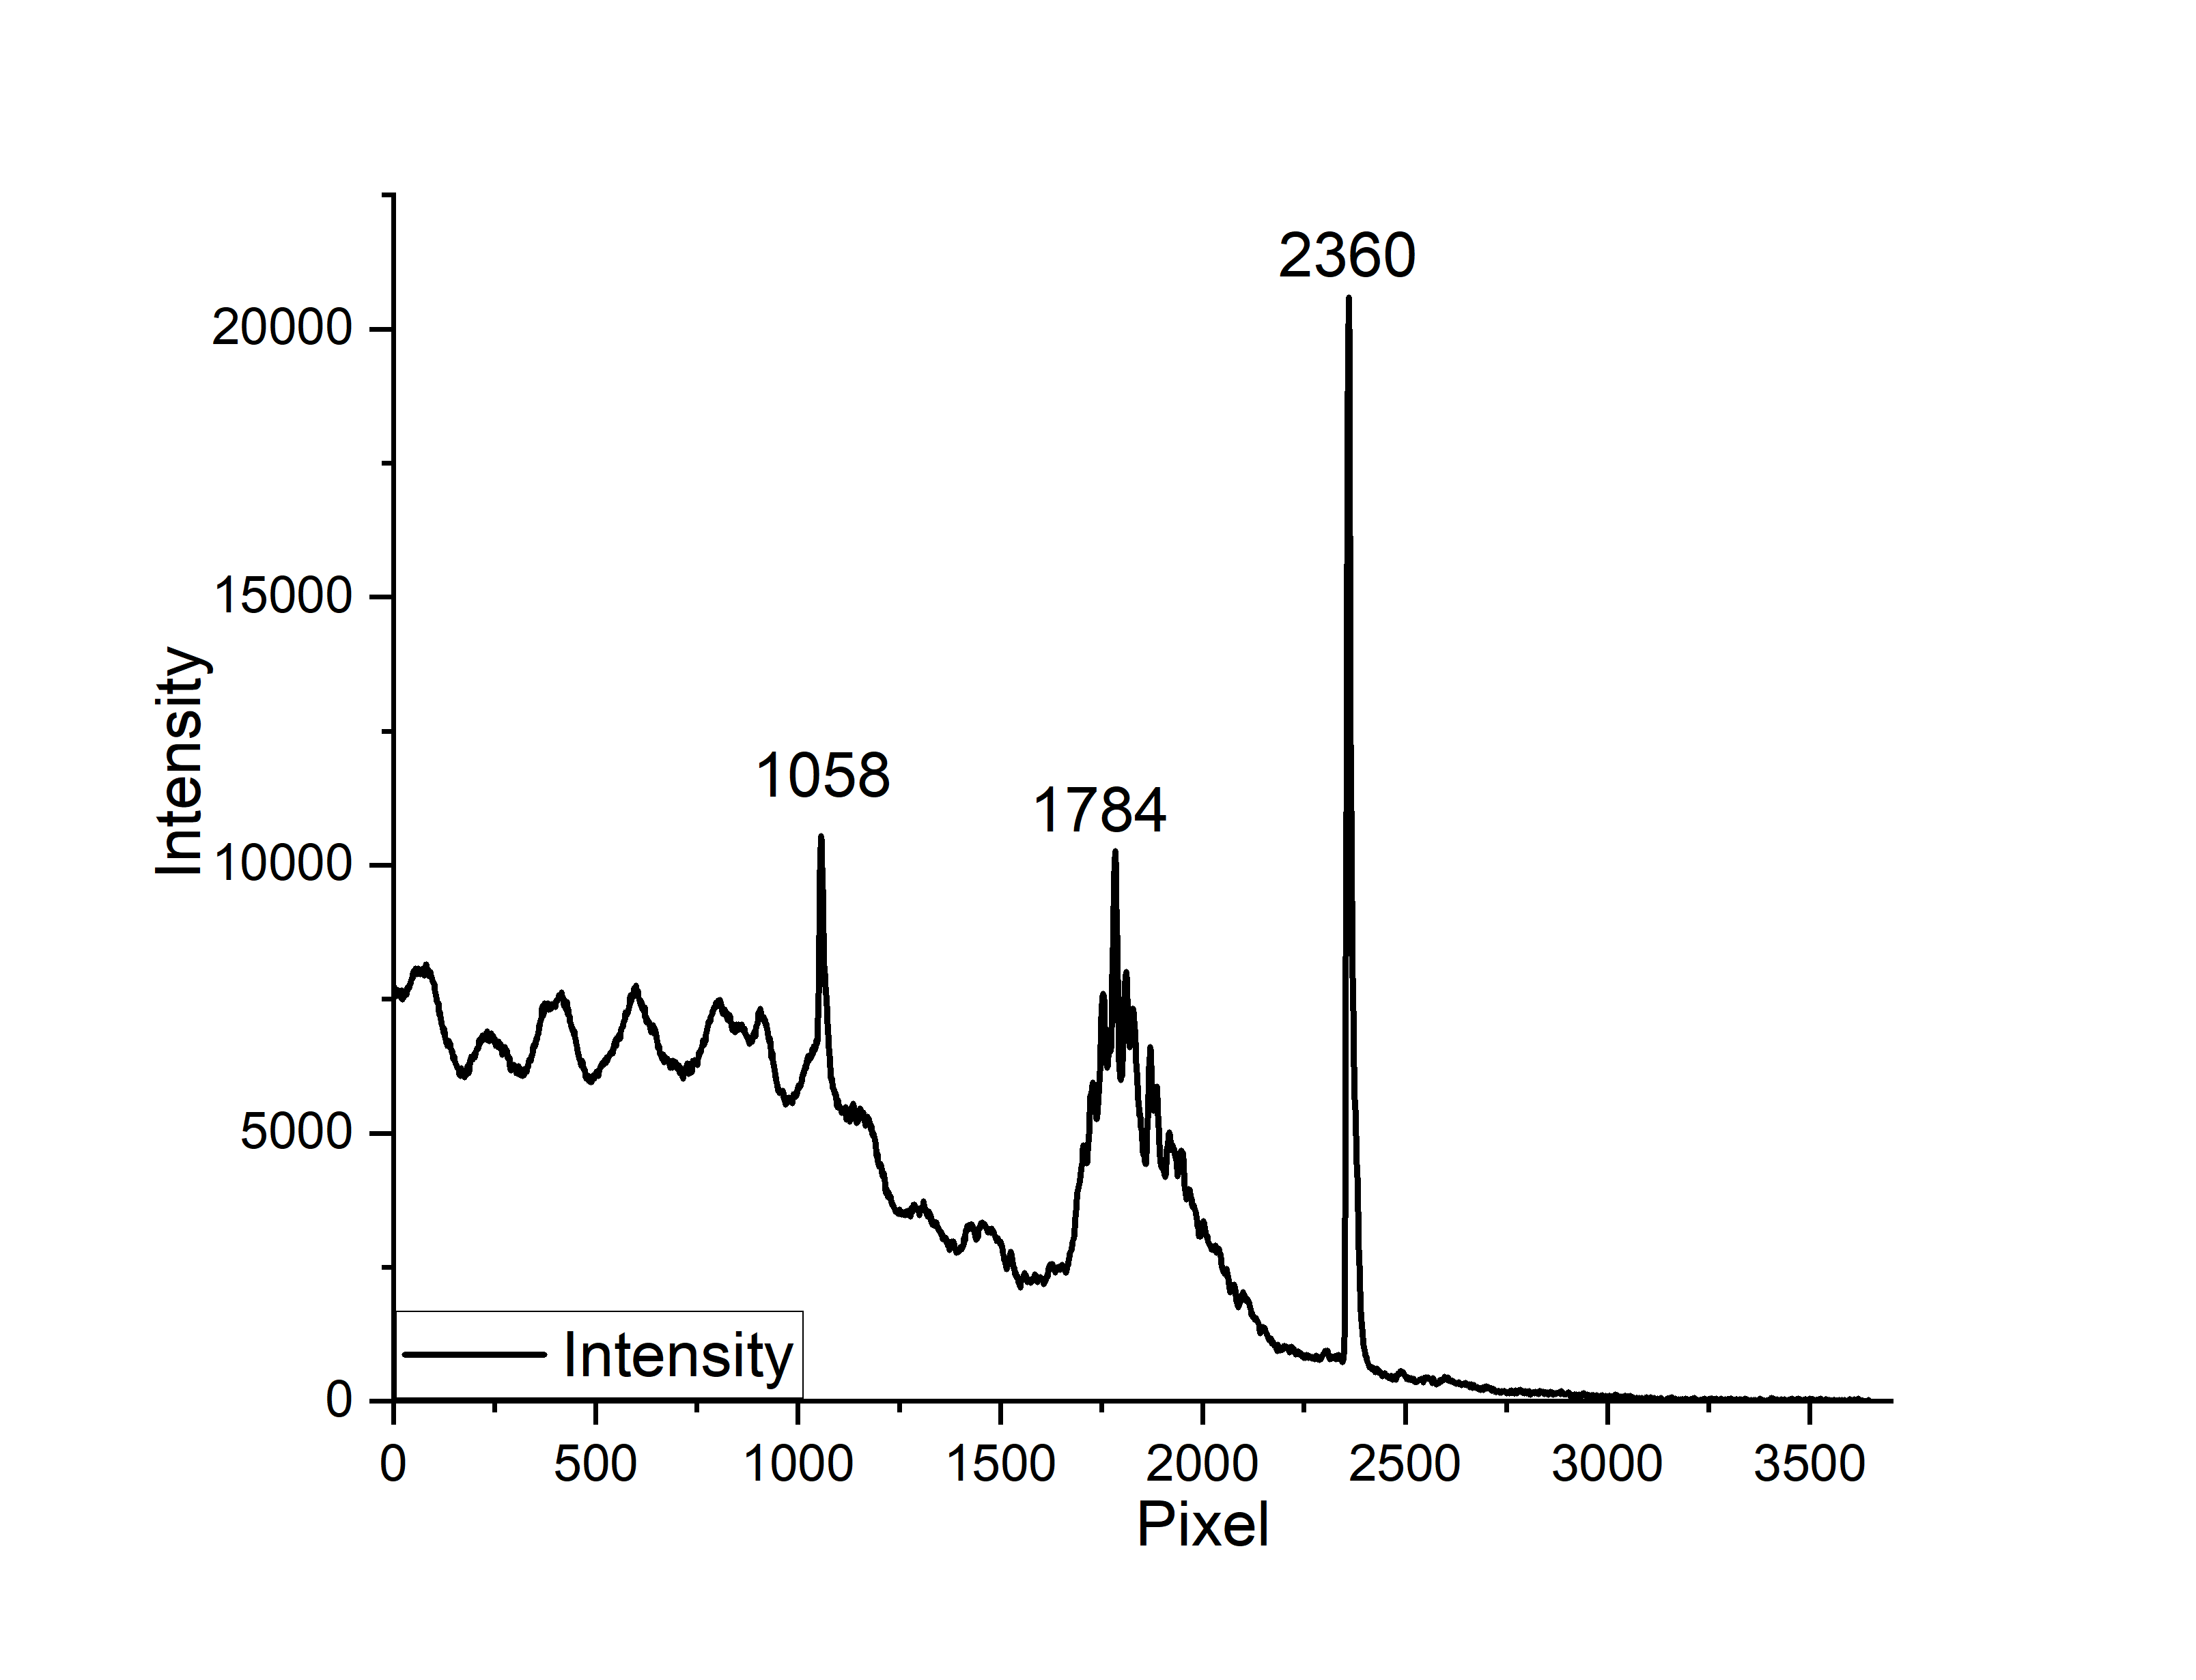
\includegraphics[width = .70\textwidth]{image/biaoding.png}
    \caption{氘灯标定下的光强-像素图}\label{5--}
\end{figure}    

\begin{figure}[htbp]
    \centering
    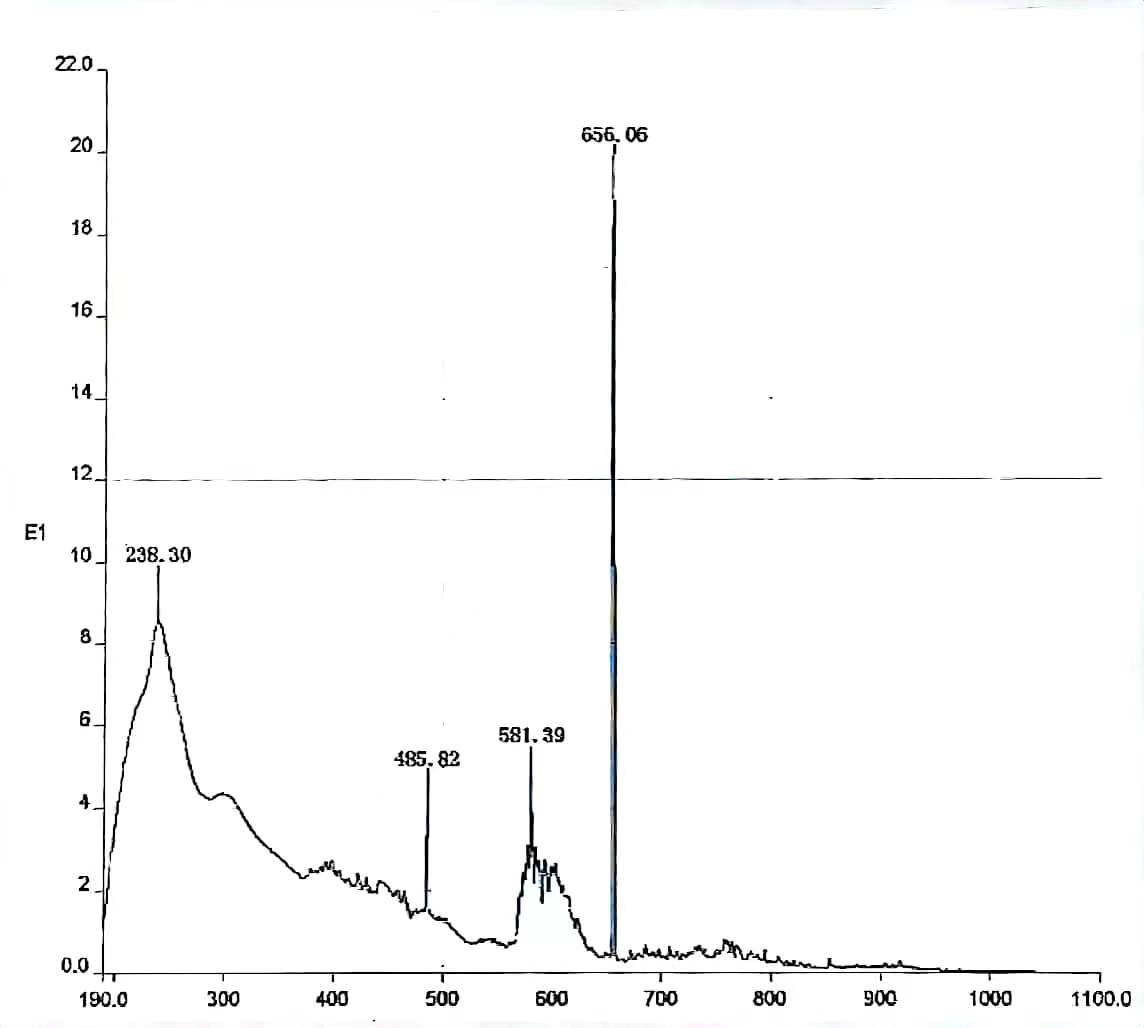
\includegraphics[width = .60\textwidth]{image/standard.jpg}
    \caption{氘灯的标准光强-像素图}\label{5-}
\end{figure} 


\begin{table}[htbp]
    \centering
    \caption{特征像素峰与标准谱对应的波长}\label{6}
    \begin{tabular}{cccc}
    \hline
            & 1      & 2      & 3      \\ \hline
    像素值     & 1058   & 1784   & 2360   \\
    \multicolumn{1}{l}{波长 $\lambda$ /nm} & 485.82 & 581.39 & 656.06 \\ \hline
    \end{tabular}
\end{table}

\begin{figure}[htbp]
    \centering
    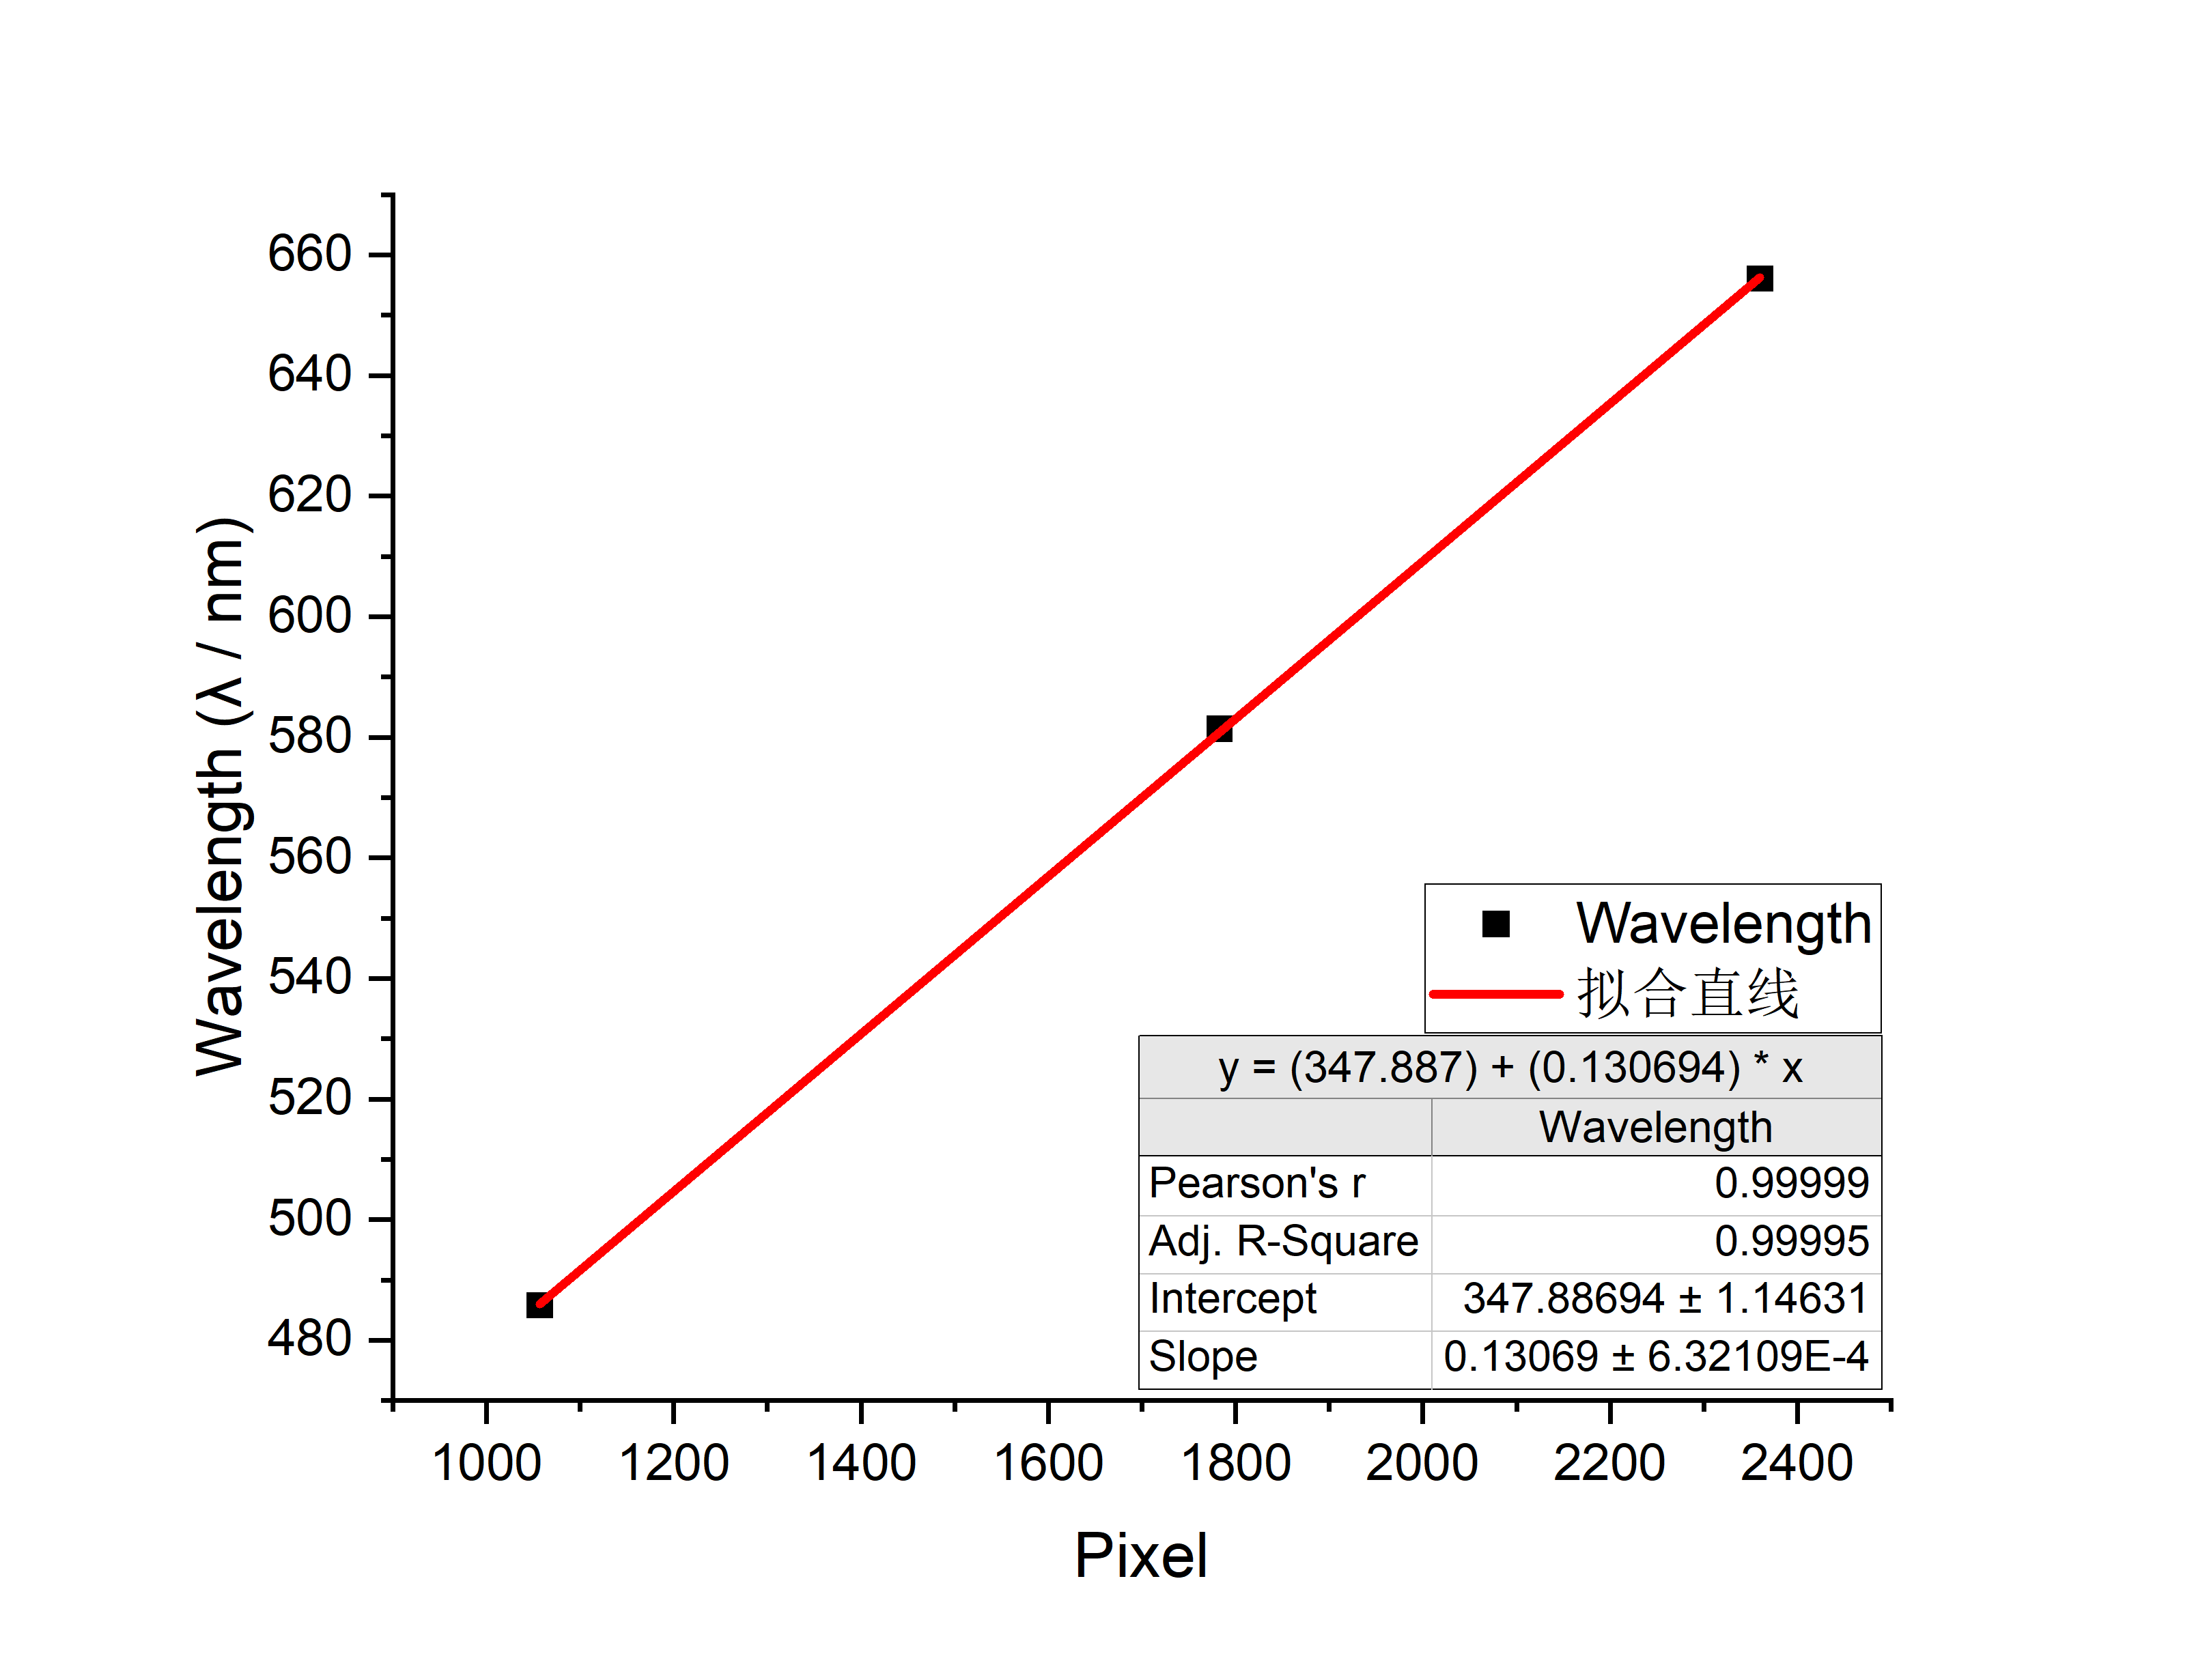
\includegraphics[width = .70\textwidth]{image/biaodingzhixian.png}
    \caption{氘灯标定标准波长-像素拟合曲线}\label{7}
\end{figure}

\newpage


\subsection{共轭分子的紫外可见吸收光谱的测定}

\subsubsection{不同浓度 A3 分子乙醇溶液的吸收光谱}

使用 3.1 中标定的紫外可见吸收光谱仪,使用卤钨灯作为光源,扣除背景后,测定空白样品
与不同浓度的 A3 分子样品的吸收光谱,得到吸收度 I 与 Pixel 的关系。通过 3.1 中的拟合曲线(\ref{nihe})与 Lambert-beer 定律
\begin{equation}\label{xgd}
    A={\rm lg}\frac{I_0}{I}=\varepsilon cb
\end{equation}

得到不同浓度 A3 分子波长与吸光度关系如图 \ref{8} 所示。观察光谱,随着浓度升高,分子的最大吸收波长几乎不变,约为 637 nm,计算
可得不同浓度下峰值吸光度如表 \ref{9} 。
\begin{table}[htbp]
    \centering
    \caption{不同浓度的 A3 分子对应的最大吸收波长和吸光度}\label{9}
    %\resizebox{ .70\textwidth}{!}
\end{table}

\begin{figure}[htbp]
    \centering
    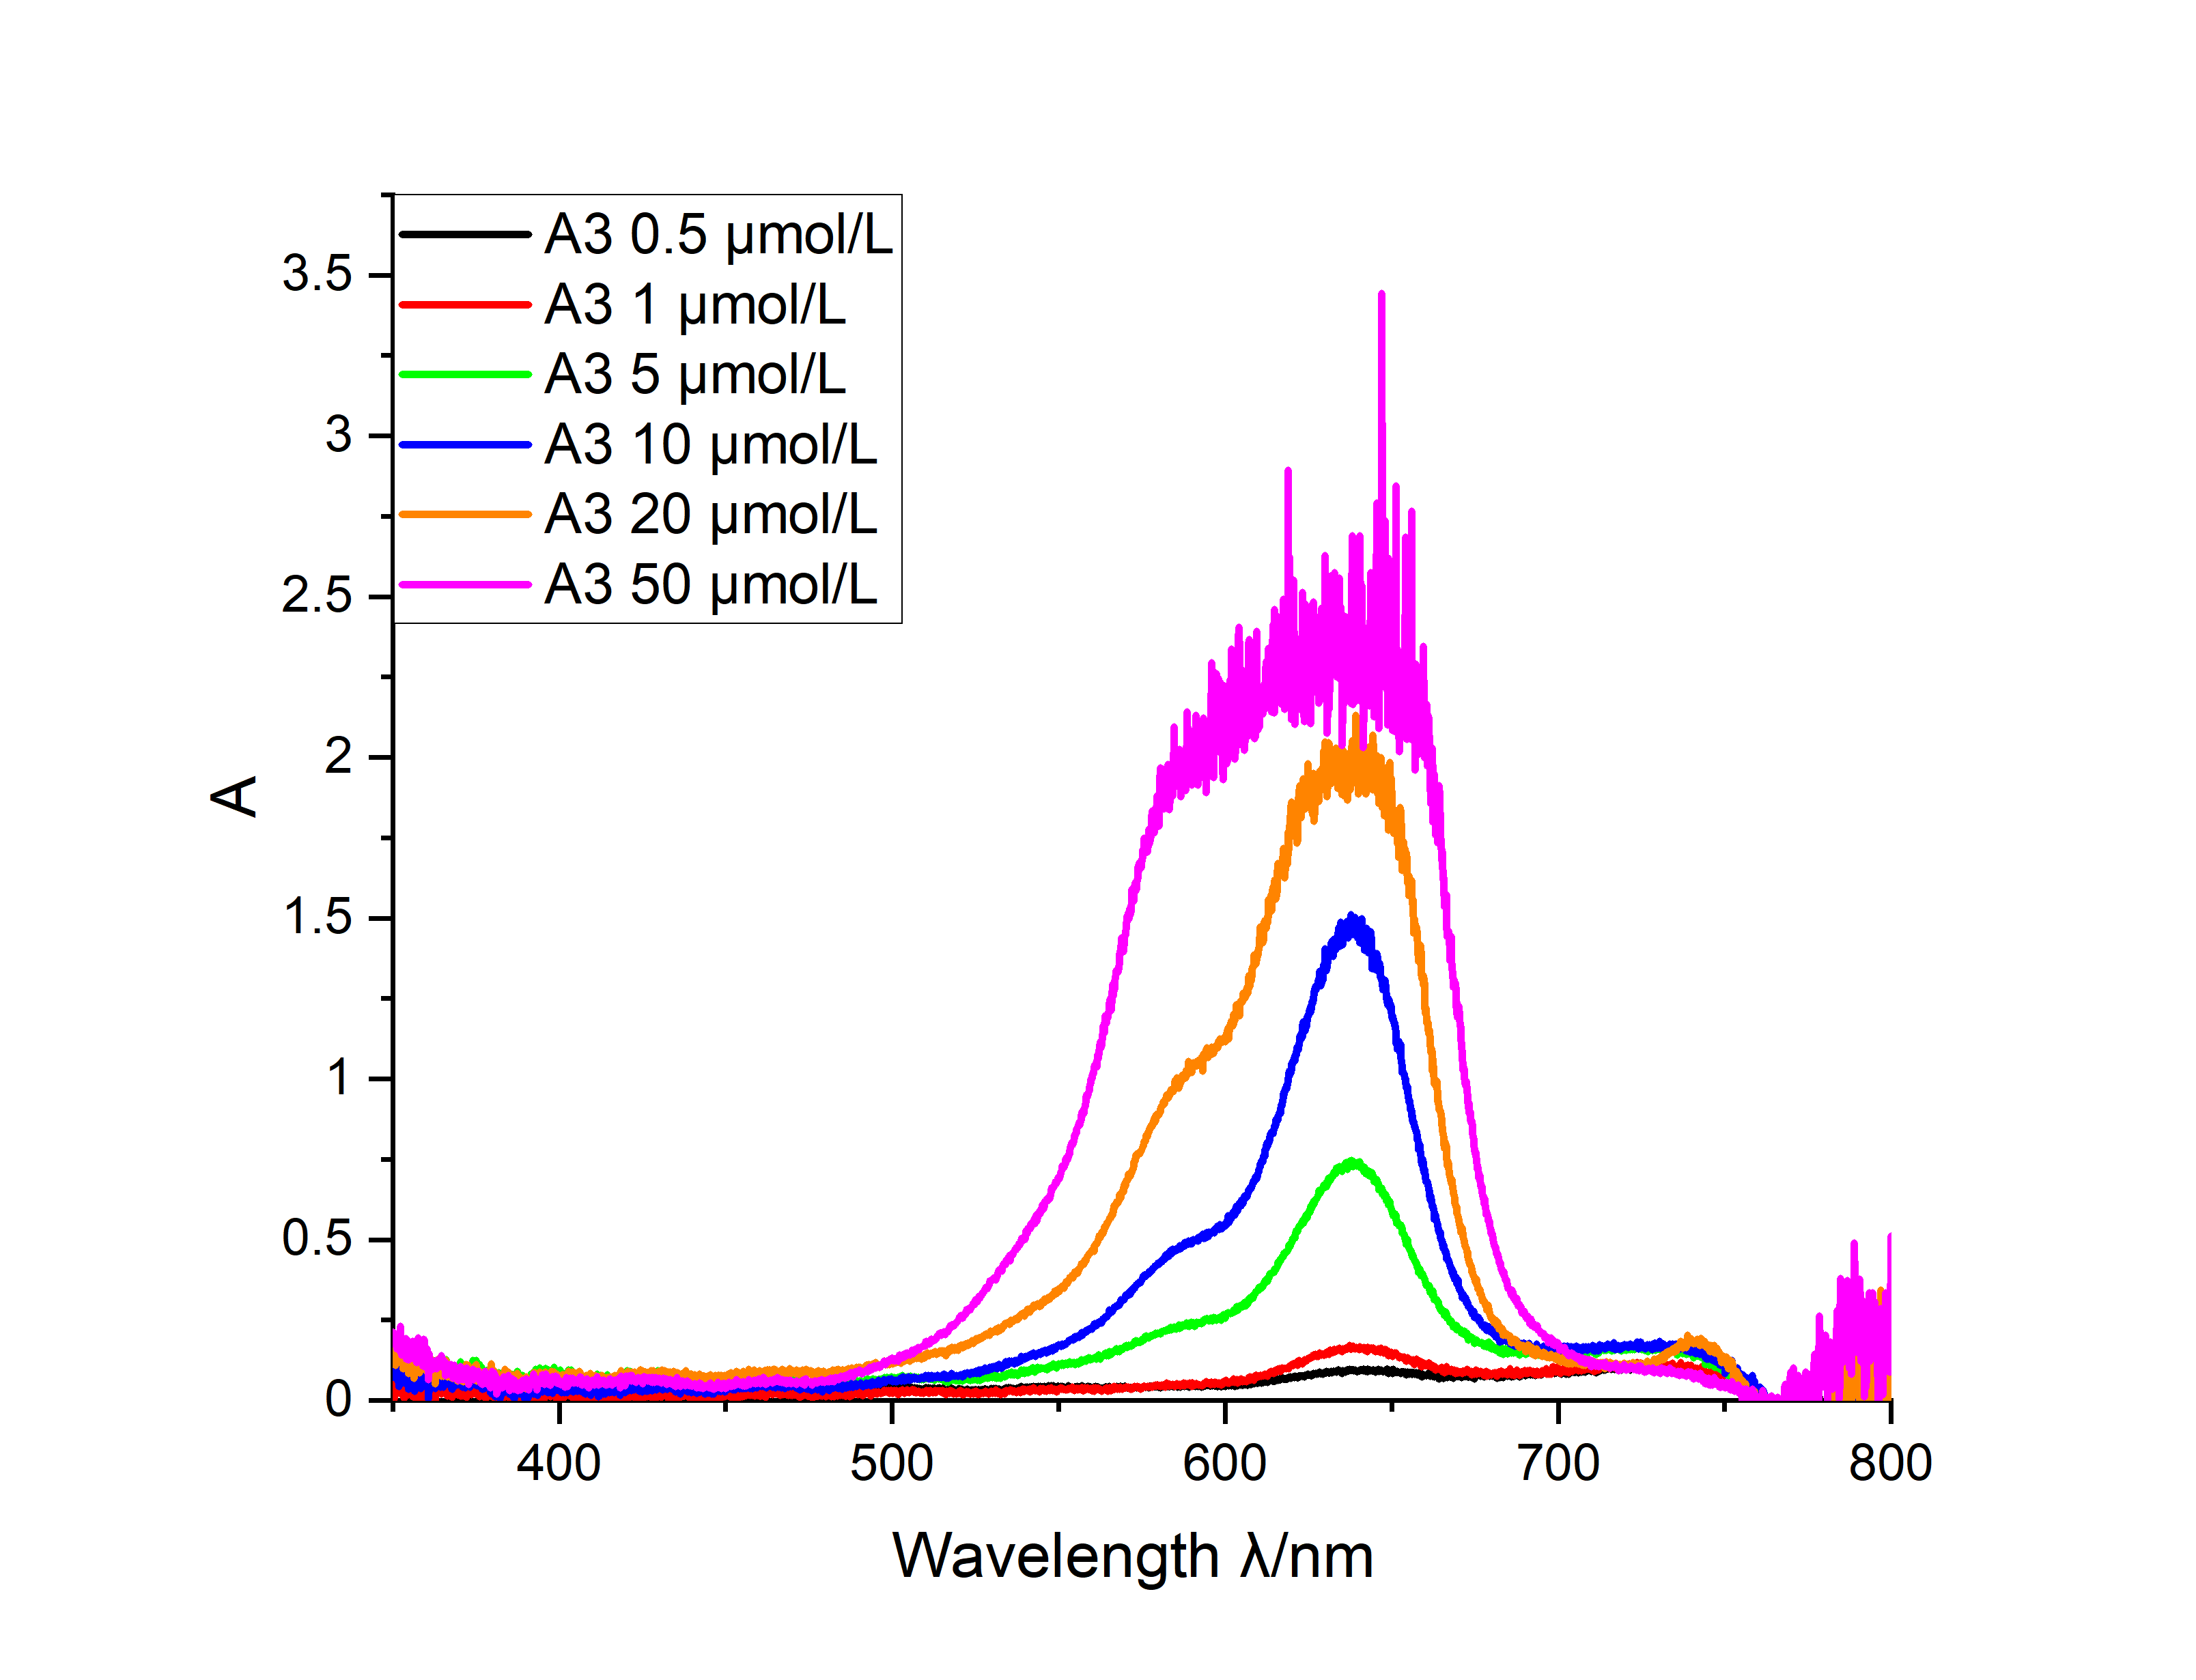
\includegraphics[width = .60\textwidth]{image/nongdu.png}
    \caption{不同浓度的 A3 分子乙醇溶液的吸收光谱}\label{8}
\end{figure}


\begin{figure}[h]
    \centering
    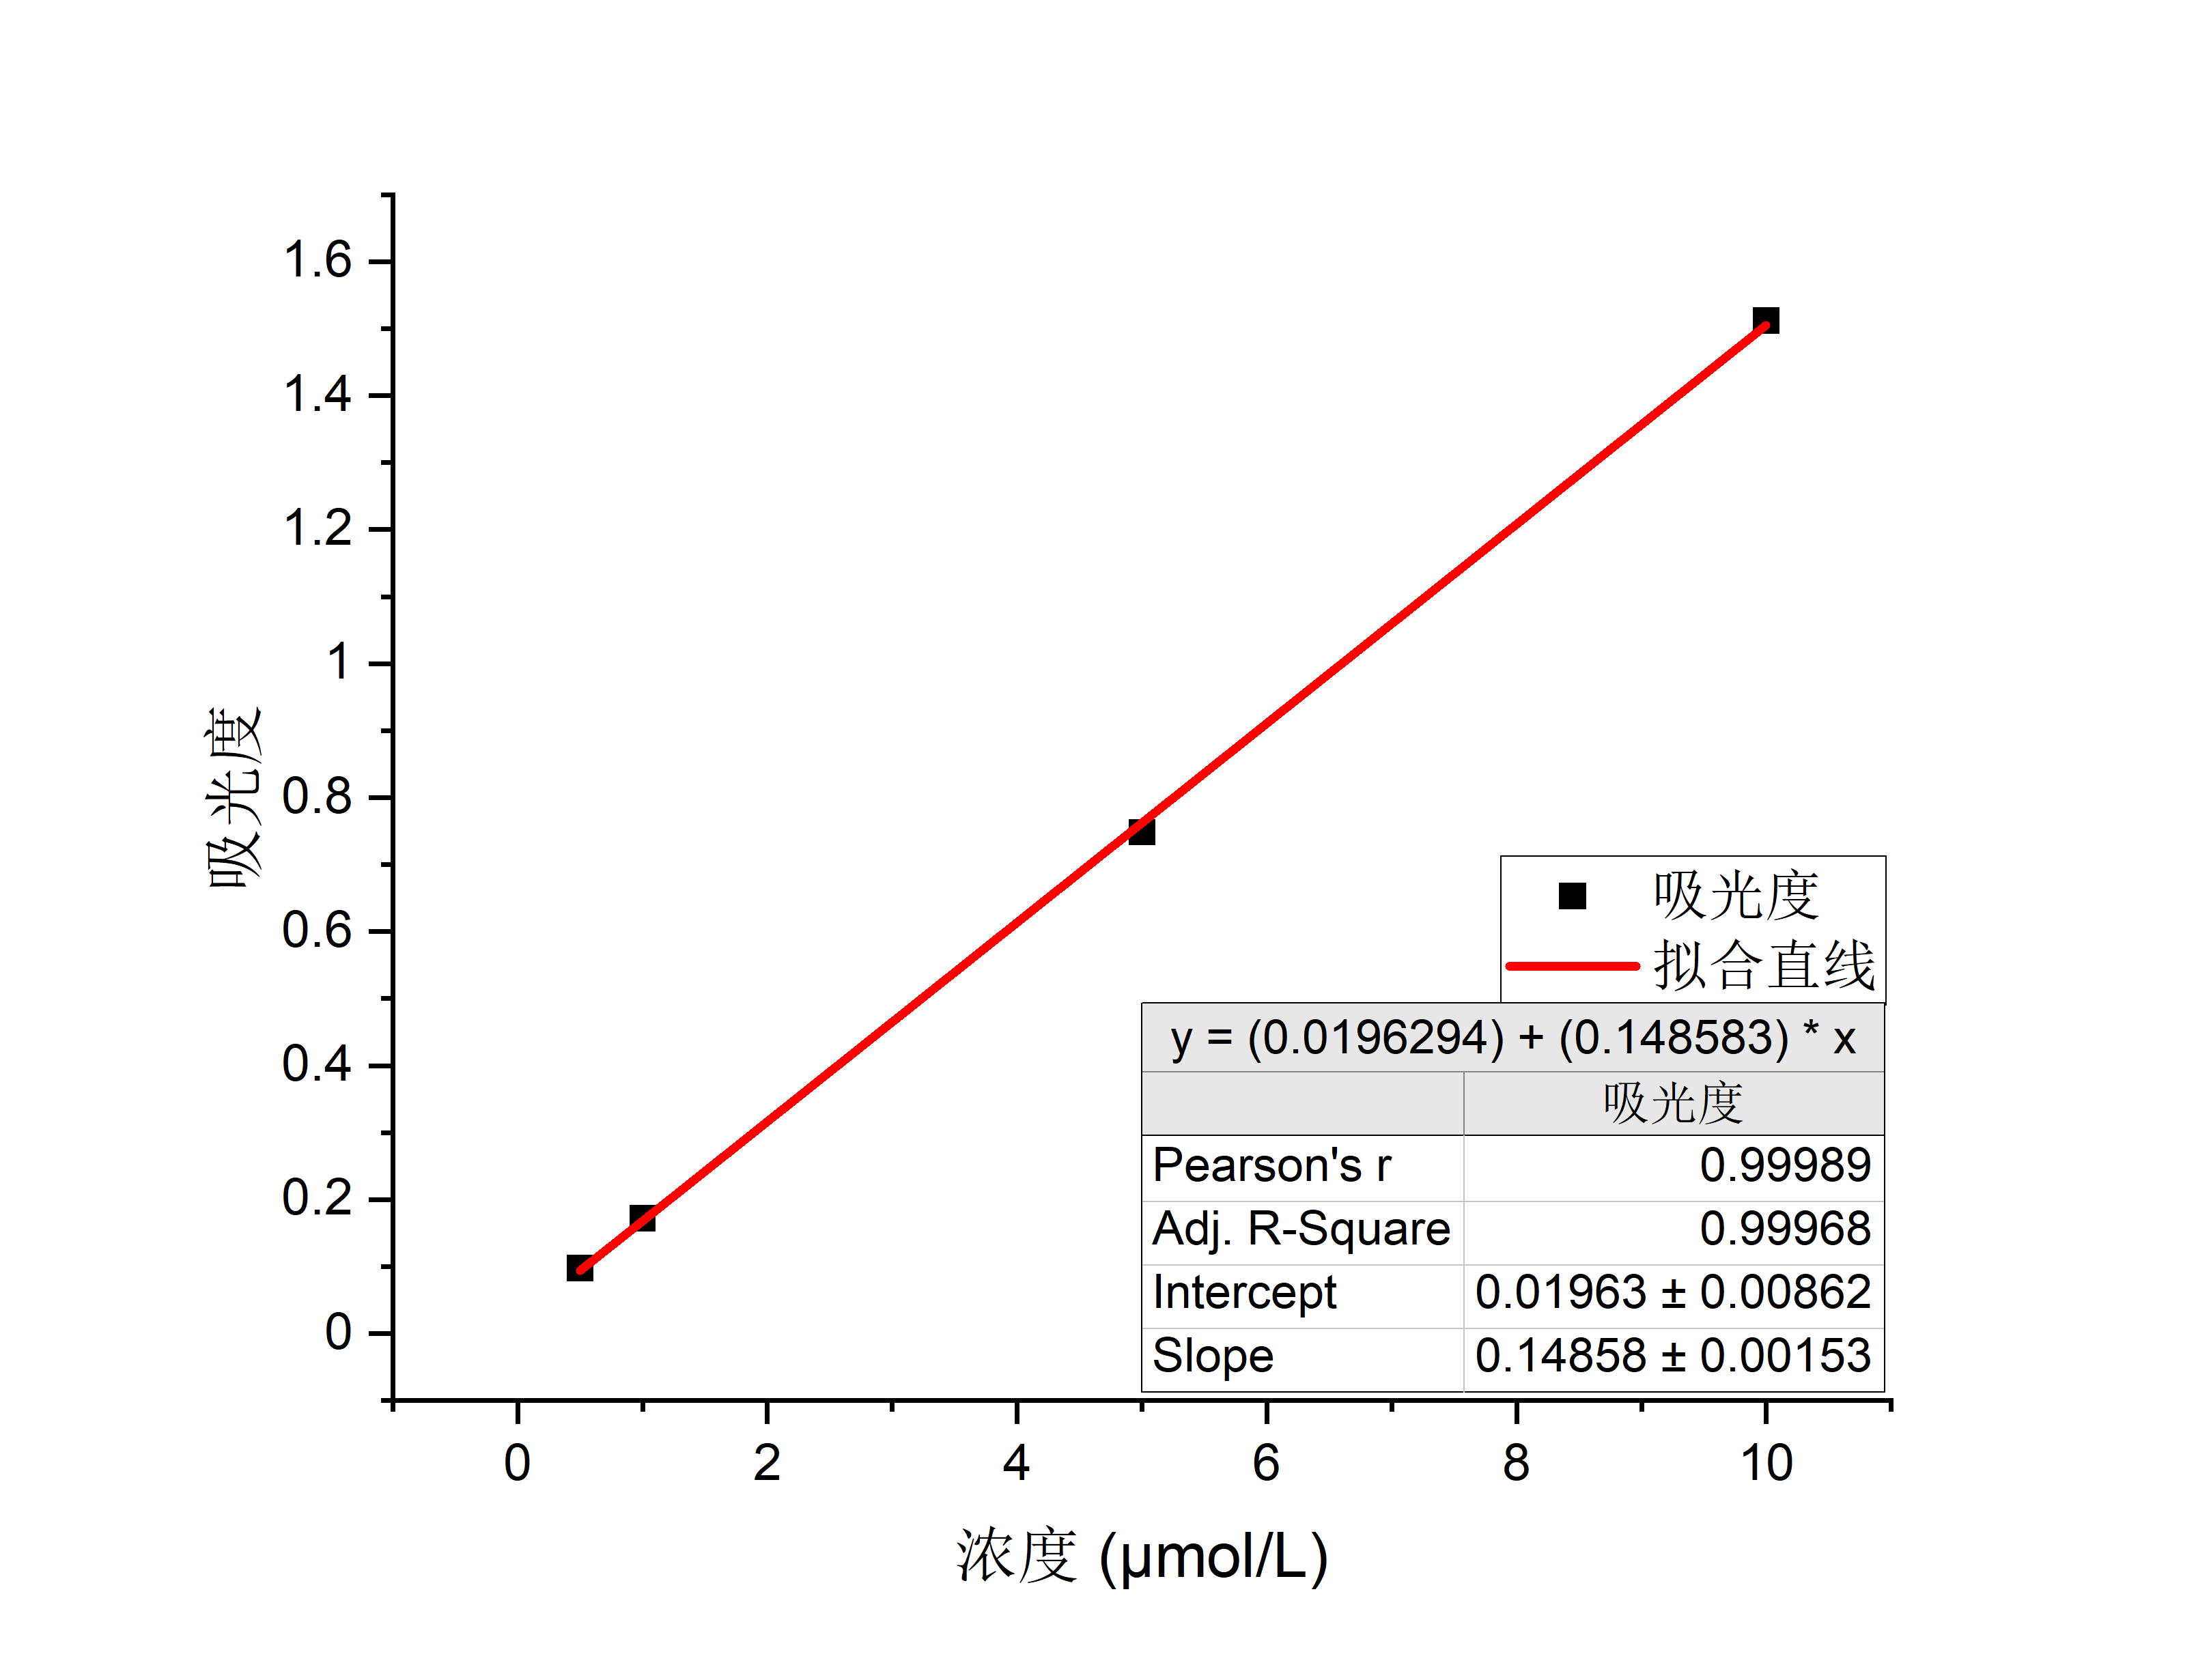
\includegraphics[width = .60\textwidth]{image/xgdzhixian.png}
    \caption{低浓度 A3 分子的浓度-吸光度拟合直线}\label{10}
\end{figure}

观察图 \ref{8} 可以发现,当浓度大于$\ 20\ \mu {\rm mol \cdot  L^{-1}}$时,由于吸光度过高,
导致图像的噪声偏大,没有有效的数据点,且不适用于 Lambert-Beer 定律,无法准确地判断峰值的吸光度。
而当浓度较小时吸光度过低,也无法准确地判断峰值的吸光度。
对低浓度的 A3 分子的吸光度进行线性拟合,得到图像如图 \ref{10} 所示,吸光度与波长的线性关系为:
\begin{equation}\label{nihe2}
    A = (0.01963 \pm 0.00862) + (0.14858 \pm 0.00153) * c \quad R^2=0.9997
\end{equation}
    
具有良好的线性关系,说明在低浓度下,吸光度与浓度成正比,符合 Lambert-Beer 定律,但是在高浓度下有偏离。
由(\ref{xgd})可以计算得到, A3 分子的摩尔吸光系数 $\varepsilon$ 为$\rm 1.49 \cdot 10^7\ L \cdot mol^{-1} \cdot m^{-1}$



\subsubsection{不同分子的吸收光谱的测定}

调节凹面镜、光栅与 CCD 的位置可以测定不同波长范围下的吸收光谱。
超出或低于光谱仪可接收的波长范围将会有较高的信噪比或无法接受到吸收光谱信号。因此我们重复标定两次紫外可见光谱,用于测定在其他波长范围有吸收峰的分子。
得到第二次氘灯标定下的光强-像素图如图 \ref{11} 和 \ref{12}。

\begin{figure}[htbp]
    \begin{minipage}{0.49\textwidth}
        \centering
        %\subfigure{
        %    \centering
        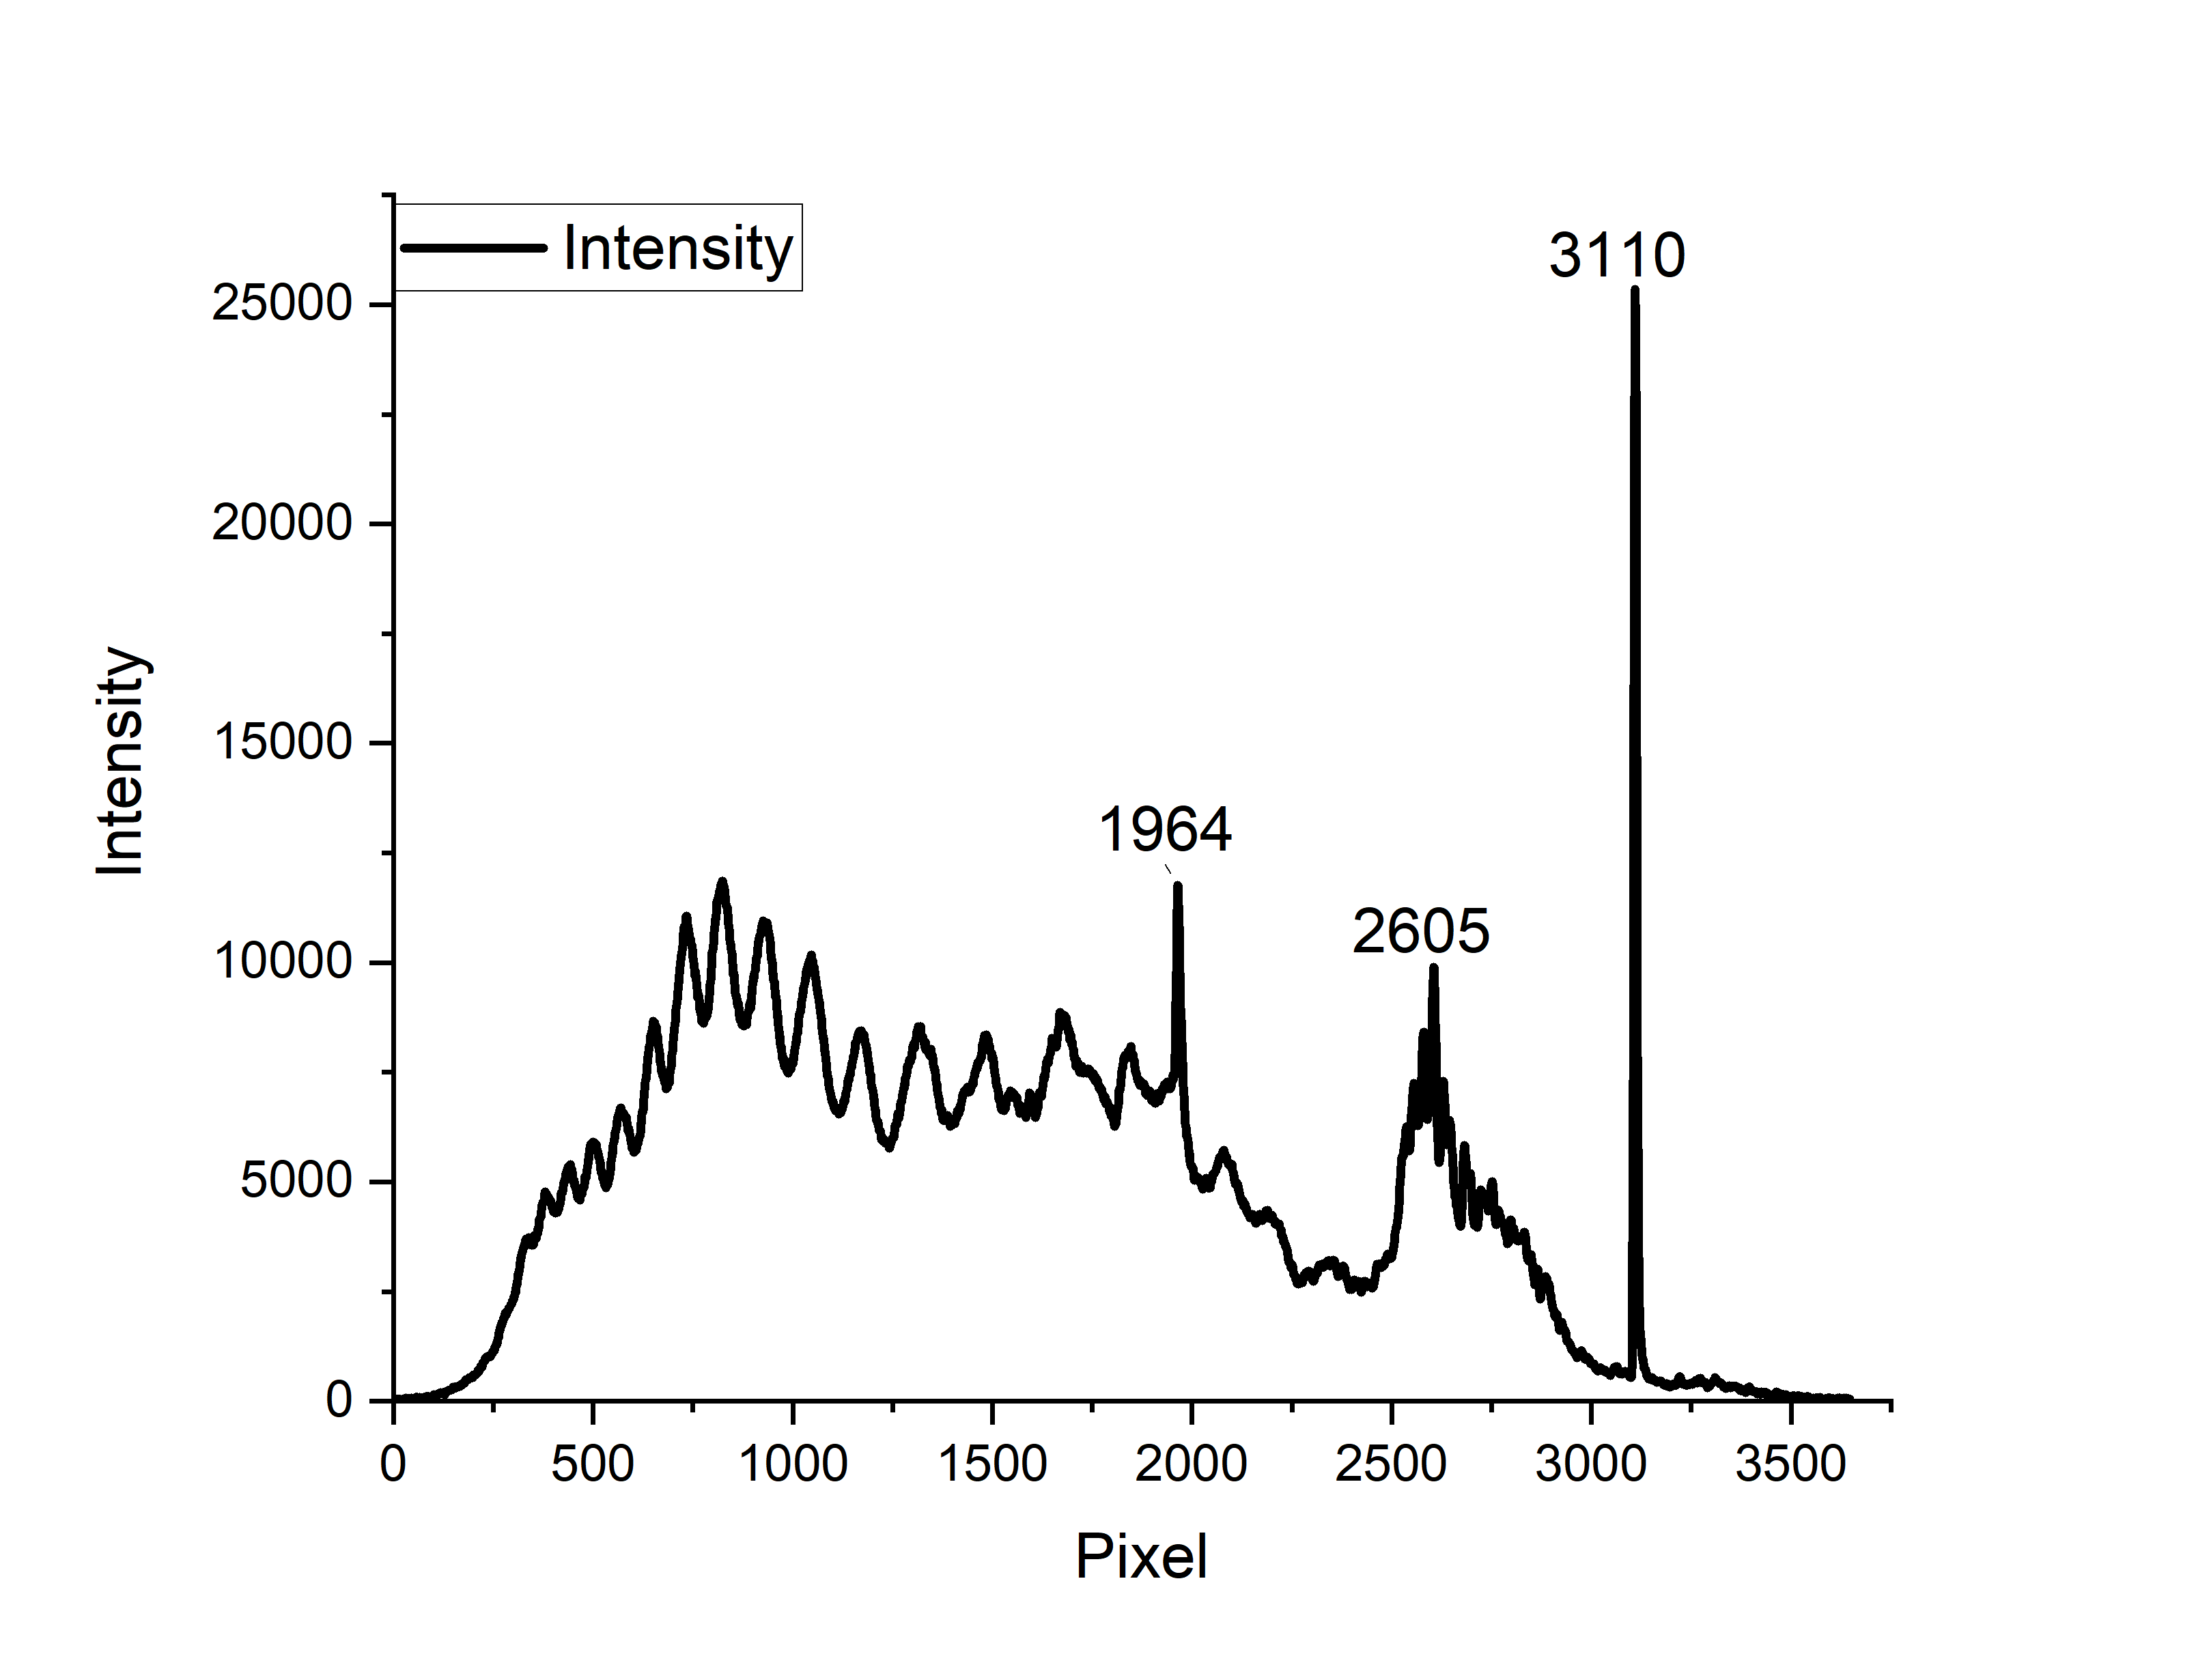
\includegraphics[height = 2.5in,width = 3.1in]{image/2biaoding.png}
        \caption{第二次氘灯标定下的光强-像素图}\label{11}
    \end{minipage}
    %}
    \centering
    %\subfigure{
    \begin{minipage}{0.49\textwidth}
        \centering
        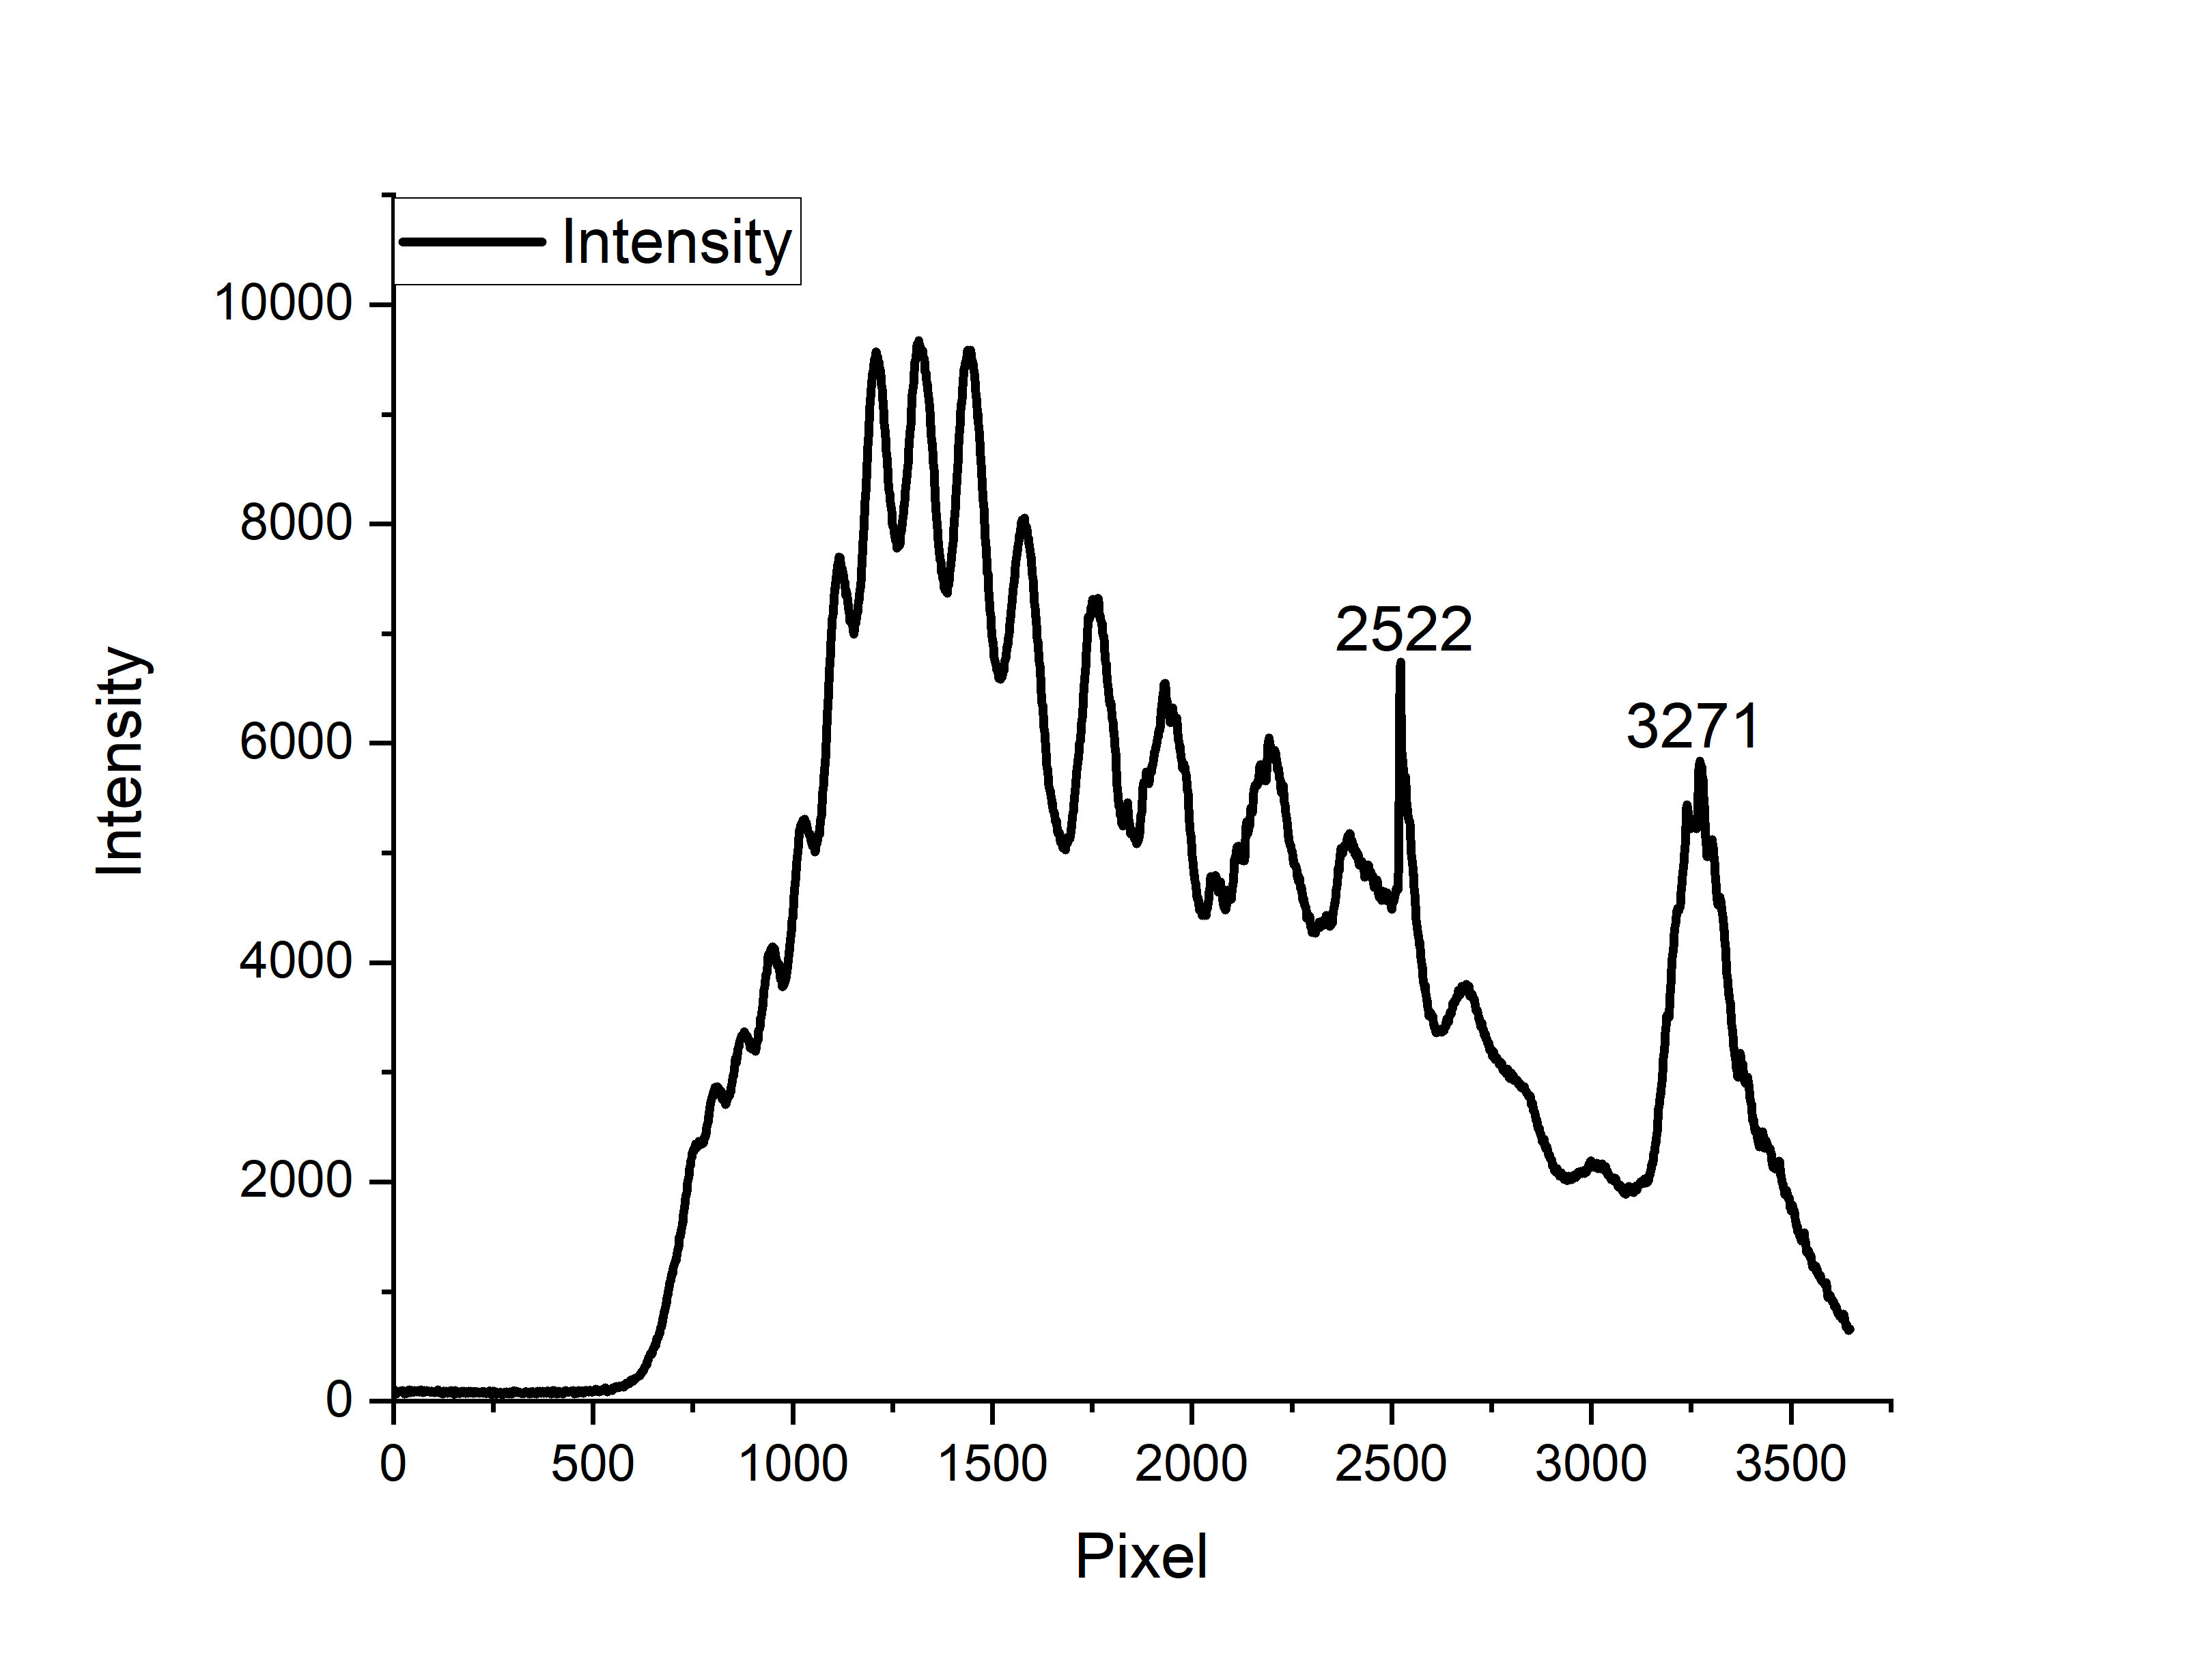
\includegraphics[height = 2.5in,width = 3.1in]{image/3biaoding.png}
        \caption{第三次氘灯标定下的光强-像素图}\label{12}
    \end{minipage}
    %}
    \centering
    %\caption{左:氘灯标定下的光强-像素图\quad右:氘灯的标准光强-像素图}\label{5}
\end{figure}

\begin{table}[htbp]
    \centering
    \caption{特征像素峰与标准谱对应的波长}\label{13}
    \begin{tabular}{cccc}
    \hline
            & 1      & 2      & 3      \\ \hline
    像素值-2     & 1964   & 2605   & 3110   \\
    像素值-3     & 2522   & 3271   & --   \\
    \multicolumn{1}{l}{波长 $\lambda$ /nm} & 485.82 & 581.39 & 656.06 \\ \hline
    \end{tabular}
\end{table}

为尽可能多地测定紫外区域的吸收峰,在第三次标定时我们舍弃了656.06 nm处的特征峰,使用两个特征峰来标定。
将两图中的特征峰与标准谱图进行比对如表 ~\ref{13} ,可以
得到 $\lambda$ 与  $ {\rm Pixel} $ 线性关系为:
\begin{equation}\label{nihe3}
    \lambda_2 = (194.11976 \pm 0.9095) + (0.14858 \pm 0.00035) * {\rm Pixel} \quad R^2=0.99996
\end{equation}
\begin{equation}\label{nihe4}
    \lambda_3 = (164.02088) + (0.1276) * {\rm Pixel}
\end{equation}

第二次标定的可测量的光谱范围为 190.27 - 736.14 nm,由于两侧的信噪比较高,实际测量范围仅为 375 nm - 730 nm。
第三次标定的可测量的光谱范围为 164.15 - 629.50 nm,实际测量范围为 240 nm - 580 nm。
我们使用第一次标定下的光谱仪测定 A3 与 A4 分子,使用第二次标定的光谱仪测定 A2 分子,使用第三次标定的光谱仪测定 A1 、B1 和 B2 分子。
得到分子的紫外可见吸收光谱如下图所示。

\begin{figure}[htbp]
    \centering
    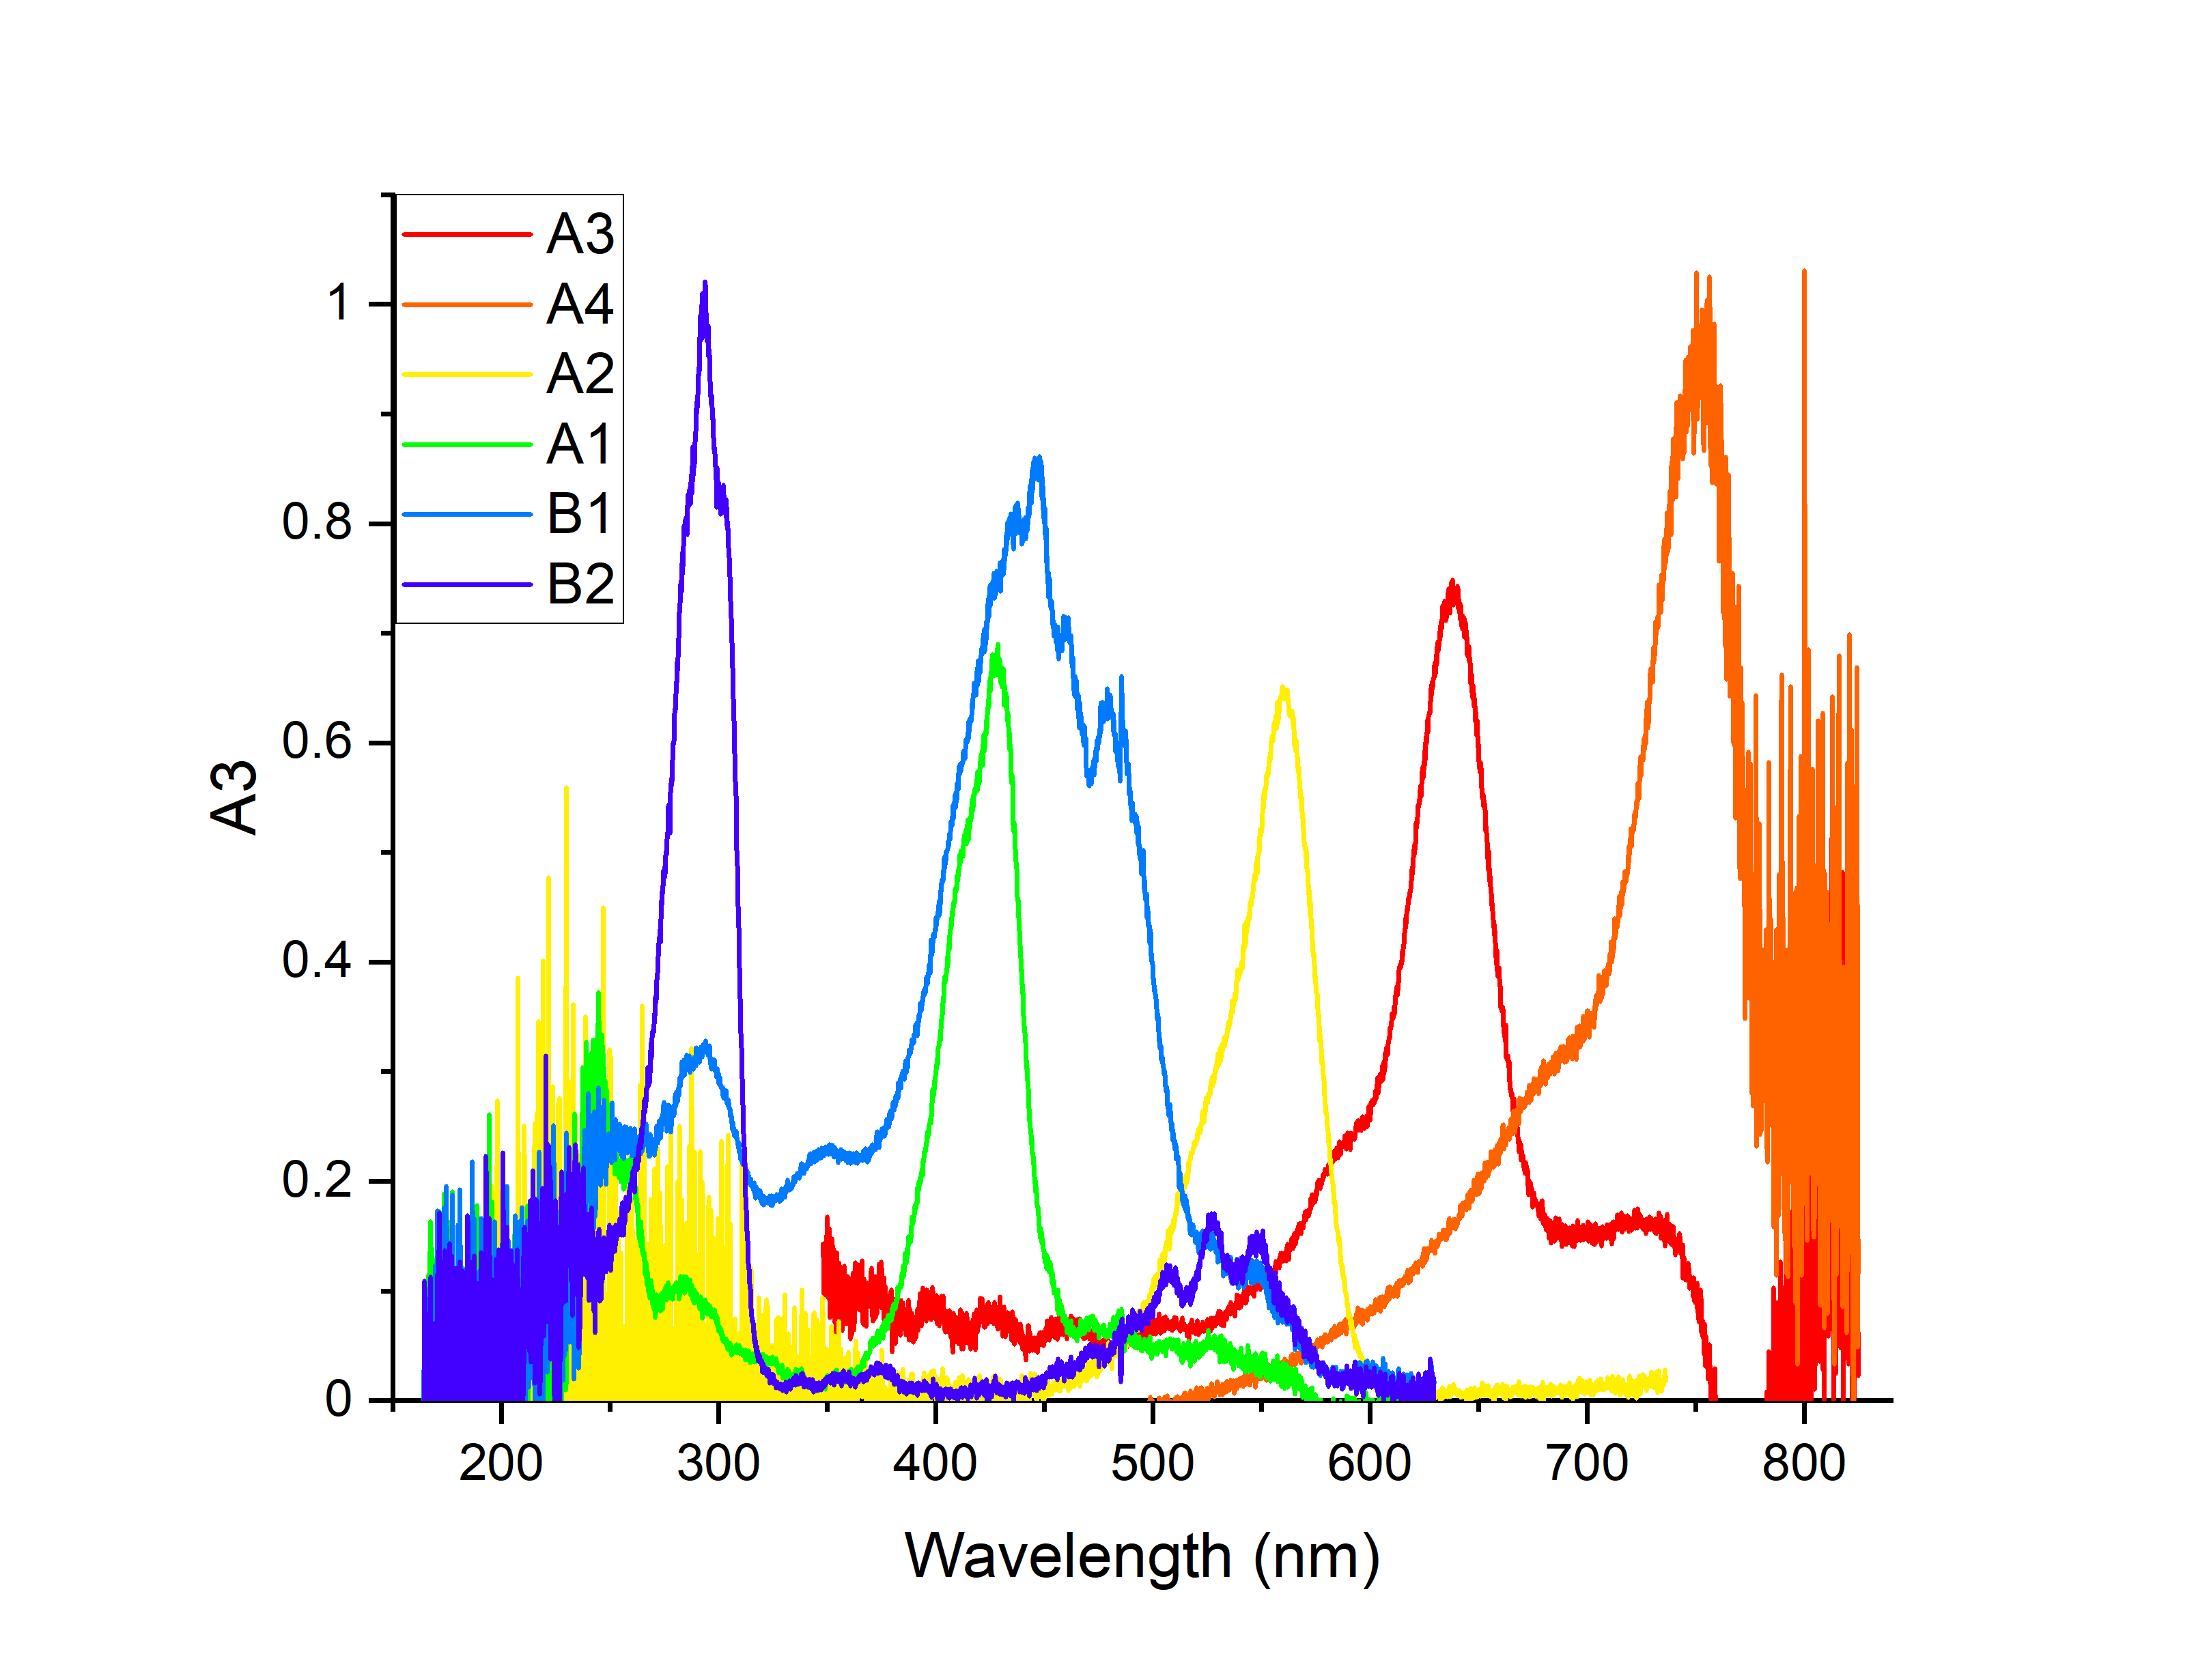
\includegraphics[width = .70\textwidth]{image/guangpu.png}
    \caption{不同分子的吸收光谱}\label{14}
\end{figure}

观察图像得到不同分子的最大吸收波长并计算其吸光度与摩尔吸光系数,如表 5 所示。对于同一组分子,随着共轭体系的增长,分子的最大吸收波长逐渐红移,摩尔吸光系数增大。
此外,对于部分分子可以观察到主峰的旁边还有副峰的存在。在 A1 分子的左侧,B1 分子的左侧和 B2 分子的右侧均可以观察到这种现象的存在,位置分别为244.79 nm,294.68 nm 和
526.92 nm。

\begin{table}[htbp]
    \centering
    \caption{不同分子的最大吸收波长与对应的吸光度}
    \label{15}
    \begin{tabular}{ccccc}
    \hline
    分子 & 波长 / nm  & 吸光度   & \multicolumn{1}{l}{浓度 / $ \mu {\rm mol \cdot  L^{-1}}$} & \multicolumn{1}{l}{$\varepsilon\ /\ {\rm 10^{6}\  L\cdot mol^{-1} \cdot m^{-1}  }$}       \\ \hline
    A1 & 428.53   & 0.690 & 10 & 6.900  \\
    A2 & 560.37   & 0.646 & 5  & 12.920 \\
    A3 & 637.35   & 0.747 & 5  & 14.940 \\
    A4 & 756.43   & 1.024 & 3  & 34.133 \\
    B1 & 445.76   & 0.860 & 10 & 8.600  \\
    B2 & 293.92   & 1.021 & 10 & 10.210 \\ \hline
    \end{tabular}
\end{table}

\subsection{一维势阱模型的验证}

由薛定谔方程
\begin{equation}
    \left(-\frac{\hbar^2}{2 m} \frac{\partial^2}{\partial x^2}+V(x)\right) \psi=E \psi
\end{equation}

在一维势阱中可得
\begin{equation}
    E=\frac{n^2h^2}{8mL^2} ,\  \Delta E=\frac{(n_1^2-n_2^2)h^2}{8mL^2}
\end{equation}

对于含有 2n 个 $\pi$ 轨道电子的线性共轭分子, $\pi$ 轨道电子可以近似认为是在一维势箱中的粒子,占据了一维势阱 n 个能级,那么最大吸收波长的势阱长度为:
\begin{equation}\label{l}
    L = \sqrt{\frac{(n_1^2-n_2^2)h^2}{8m\Delta E}} =  \sqrt{\frac{(2n + 1)h\lambda_{max}}{8mc}}
\end{equation}

A 组分子通式如下图所示。若考虑苯环对线性共轭分子的影响,那么显然不满足一维势箱模型。因此线性共轭分子的 $\pi$ 
电子个数主要受到噻唑环参与共轭电子对数的影响。因此有 $k+1$ 至 $k+3$ 三种情况。

\begin{figure}[htbp]
    \centering
    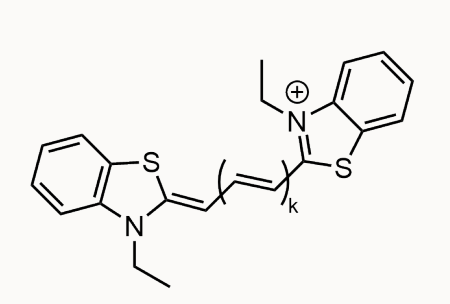
\includegraphics[width = .30\textwidth]{image/amol.png}
    \caption{A 组分子的通式}\label{16}
\end{figure}

共轭烯烃中,碳碳双键键长为$\rm 1.34\ \mathring{A} $,碳碳单键键长为$\rm 1.48\ \mathring{A} $,因此可以假设在分子中
碳碳键的平均长度为$\rm 1.41\ \mathring{A}$。考虑 A 组分子中的共轭电子对数为 $k+1$ 至 $k+3$ 的情况,如下表 \ref{17} 所示,并计算一维势阱理论模型的结果如表 \ref{18} 。

\begin{table}[h]
    \centering
    \caption{A 组分子一维势阱模型的势阱长度}
    \label{17}
    \begin{tabular}{cccccc}
    \hline
    \multicolumn{1}{l}{\multirow{2}{*}{分子}} & \multicolumn{1}{l}{\multirow{2}{*}{最大吸收波长 / nm}} & \multicolumn{1}{l}{\multirow{2}{*}{$k$}} & \multicolumn{3}{c}{势阱长度 /$\rm \ \mathring{A} $} \\
    \multicolumn{1}{l}{}                    & \multicolumn{1}{l}{}                             & \multicolumn{1}{l}{}                   & $n=k+1$   & $n=k+2$  & $n=k+3$  \\ \hline
    A1 & 428.53 & 0 & 6.242  & 7.208  & 15.069 \\
    A2 & 560.37 & 1 & 9.215  & 10.094 & 19.948 \\
    A3 & 637.35 & 2 & 11.628 & 12.431 & 23.362 \\
    A4 & 756.43 & 3 & 14.364 & 15.141 & 27.807 \\ \hline
    \end{tabular}
\end{table}

\begin{table}[h]
    \centering
    \caption{不同电子对数对应的势阱长度}
    \label{18}
    \begin{tabular}{lcccccccc}
    \hline
    \multicolumn{1}{c}{n}       & 1    & 2    & 3    & 4     & 5     & 6     & 7   & 11  \\\hline
    势阱长度 /$\rm \ \mathring{A} $ & 4.23 & 7.05 & 9.87 & 12.69 & 15.51 & 18.33 & 21.15 & 32.43\\\hline
    \end{tabular}
\end{table}


两者对比得到理论与实际势阱长度差如表 \ref{19}。可以看出,当采用 $n=k+2$ 时,理论计算与实际势阱长度差异较小,平均差异为 $\rm 0.253\ \mathring{A}$,而当电子对为其他数量时差异较大。
考虑到键长差异等误差影响,A 组分子可以近似看作所有芳环外的双键参与形成的一维势箱,一维势箱理论模型可以较好描述 A 组分子。


\begin{table}[h]
    \centering
    \caption{理论与实际势阱长度差异}
    \label{19}
    \begin{tabular}{ccccc}
    \hline
    \multicolumn{1}{l}{\multirow{2}{*}{分子}} & \multicolumn{1}{l}{\multirow{2}{*}{$k$}} & \multicolumn{3}{c}{势阱长度差 /$\rm \ \mathring{A} $} \\
    \multicolumn{1}{l}{}                    & \multicolumn{1}{l}{}                     & $n=k+1$     & $n=k+2$    & $n=k+3$    \\ \hline
    A1 & 0 & 2.012 & 0.158  & 0.956  \\
    A2 & 1 & 2.165 & 0.224  & -0.102 \\
    A3 & 2 & 1.758 & -0.259 & -2.684 \\
    A4 & 3 & 1.674 & -0.369 & -4.496 \\ \hline
    \end{tabular}
\end{table}

\newpage

B组分子为纯碳碳双键,由(\ref{l})计算可以得到

\begin{equation}
    L_{B1, n=11} =  \sqrt{\frac{(2n + 1)h\lambda_{max}}{8mc}} = 17.627{\rm \ \mathring{A}}
\end{equation}

\begin{equation}
    L_{B2, n=3} =  \sqrt{\frac{(2n + 1)h\lambda_{max}}{8mc}} = 7.896{\rm \ \mathring{A}}
\end{equation}

与表 \ref{18} 相对比,发现两个分子实际与理论计算的差别均较大。$\Delta L_{B1} = |32.43 - 17.624| = 14.81{\rm \ \mathring{A}},\ \Delta L_{B2} = |9.87 - 7.896|  = 1.97{\rm \ \mathring{A}} $
因此一维势箱理论模型不能描述 B 组分子。

综上所述,一维势箱理论模型可以较好地描述 A 组硫菁碘盐类分子,但是不能很好地估测由单纯共轭碳碳键形成的B组分子。

\subsection{理论计算}

由于设备的客观因素,使用较大的基组与复杂的泛函将会消耗大量的时间。若使用 B3LYP 泛函与 6-31g(d) 基组,在不考虑溶剂化作用计算A2分子将会消耗1个小时以上的时间
因此本次理论计算考虑使用半经验方法 AM1 进行结构优化,再使用相同的方法优化激发态几何结构,得到结果如下表 \ref{22}。


\begin{table}[h]
    \centering
    \caption{使用 AM1 方法计算 A 组与 B 组分子最大吸收波长}
    \label{22}
    \begin{tabular}{ccccccc}
    \hline
       &  能量差 / Hartree & 波长 / nm & 实际波长 / nm & 波长差 / nm \\ \hline
    A1 &  0.062         & 736.41  & 428.53    & 307.88   \\
    A2 &  0.065         & 703.89  & 560.37    & 143.52   \\
    A3 &  0.057         & 802.49  & 637.35    & 165.14   \\
    A4 &  0.050         & 909.66  & 756.43    & 153.23   \\
    B1 &  0.087         & 579.55  & 445.76    & 133.79    \\
    B2 &  0.122         & 403.13  & 293.92    & 109.21    \\ \hline
    \end{tabular}
\end{table}

可以看出,通过半经验方法得到的波长结果与实际有显著的区别,差距一般在 130 nm 左右。在 A1 分子中,由于 N 上的乙基使得整个分子较为拥挤
。为得到相对可靠的结果,将两个乙基调整为顺式结构,否则将会产生更大的误差。比较 A2 - A4 分子的计算波长可以发现,相邻分子的波长差(如$\lambda_{A3}-\lambda_{A4}$)与实际结果较为吻合,波长差较为稳定,
具有明显的单调性,由此可以说明这样的理论计算结果也可以支持一维势箱近似的结论。但是用这种方法计算得到A组分子误差实在过大,做出紫外可见光谱图与进一步的讨论
没有实际意义。

我们使用 Multiwfn 软件对如上的 B1 与 B2 分子计算紫外可见光谱图,如下图 \ref{b1} 与 \ref{b2} 所示。\cite{DBLP:journals/jcc/LuC12}

\begin{figure}[htbp]
    \centering
    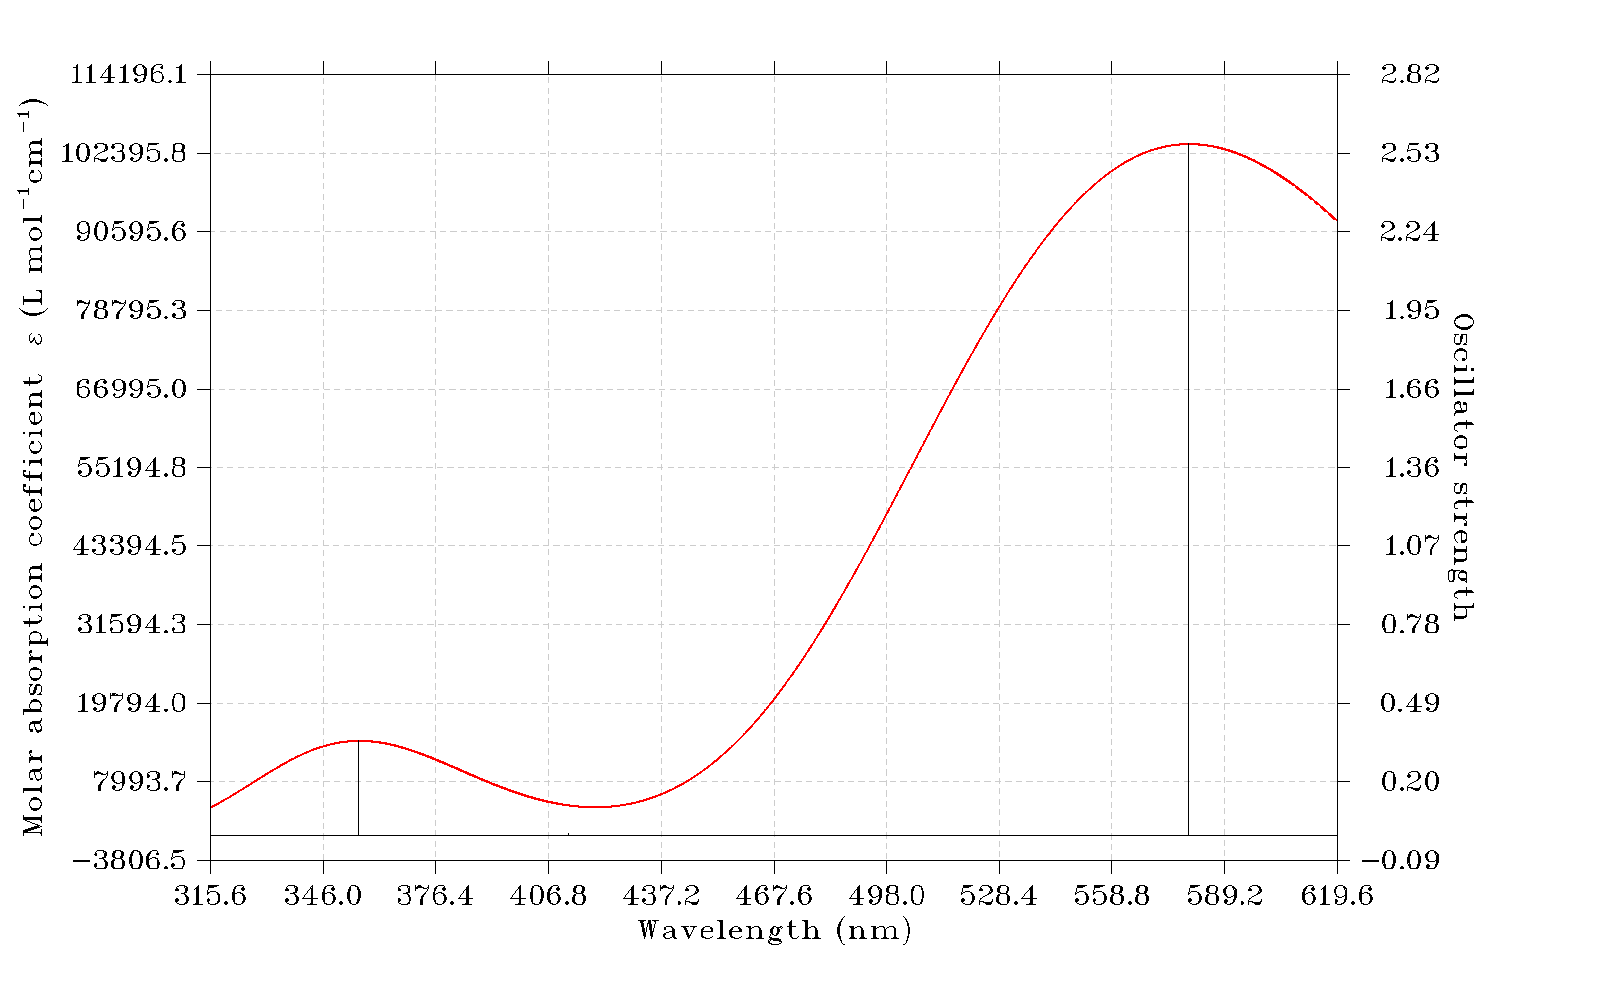
\includegraphics[width = .70\textwidth]{image/B1.png}
    \caption{B1 分子紫外可见光谱图}\label{b1}
\end{figure}
\begin{figure}[htbp]
    \centering
    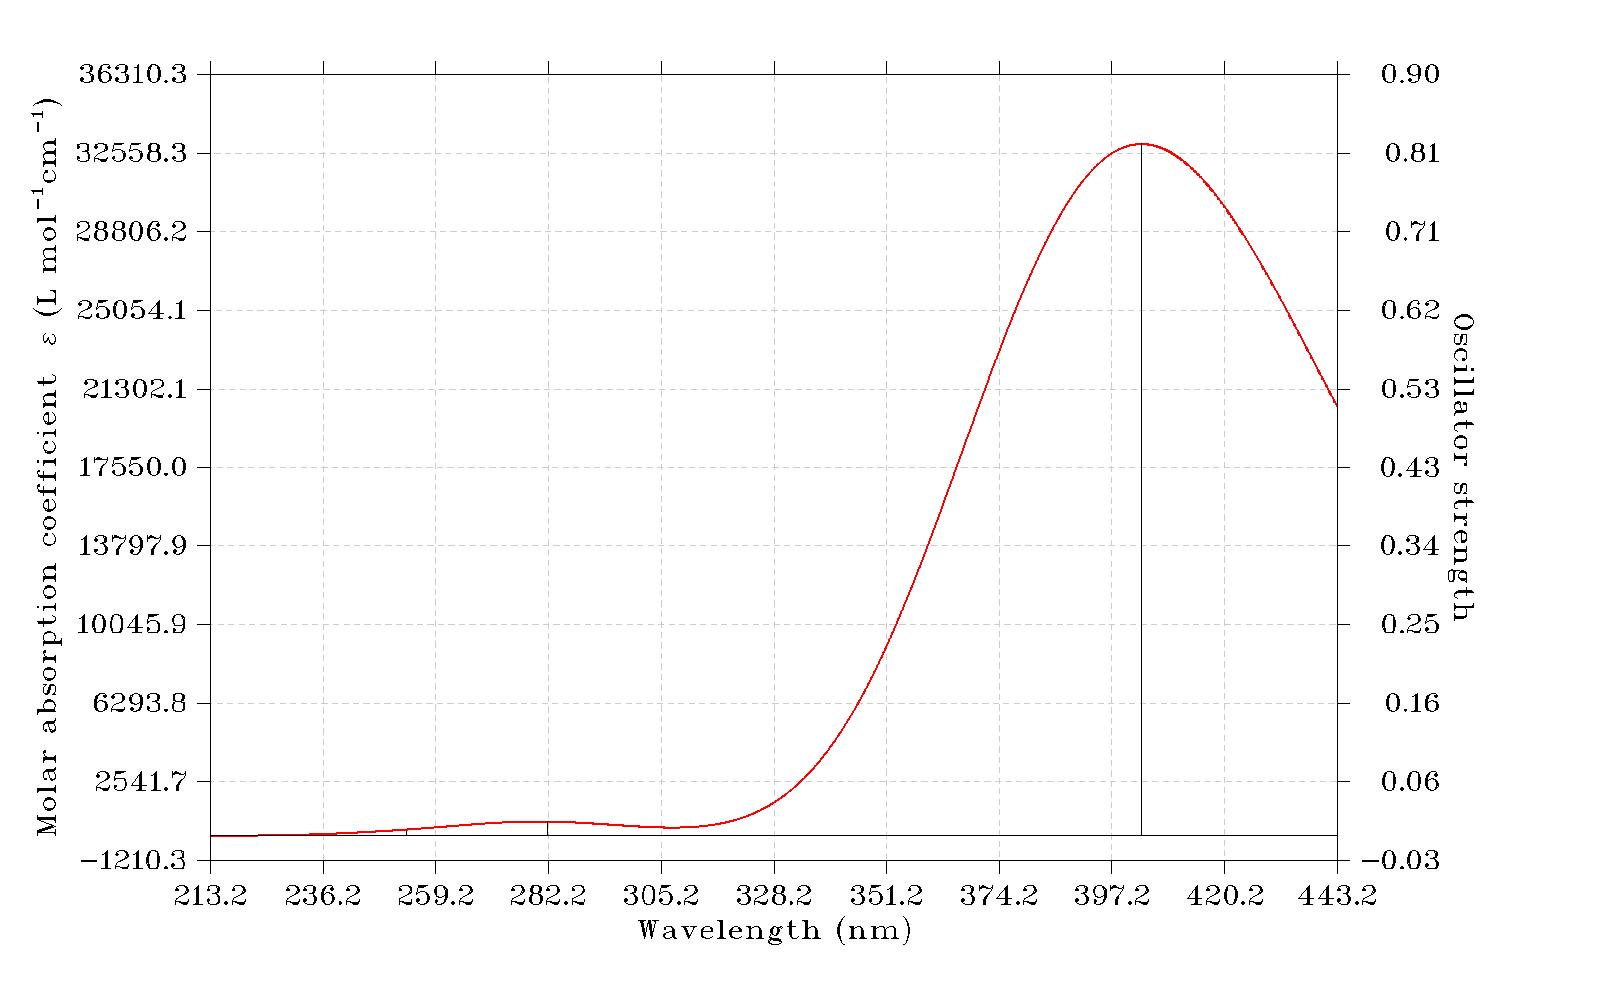
\includegraphics[width = .70\textwidth]{image/B2.png}
    \caption{B2 分子紫外可见光谱图}\label{b2}
\end{figure}

注意到两图中在光谱左侧还存在一个肩峰,这一点可以在实际测量的 B1 光谱图中观测到,说明使用这一计算方法对于纯碳链的共轭双键的计算是有一定参考意义的。
而对于这些分子在有充足计算资源的情况下应当如何计算,将在讨论部分进行进一步阐述。

%b1 579.5460
%b2 403.1346


\section{实验结果与讨论}

\subsection{讨论}

\subsubsection{吸光度的选择}

由 Lambert-Beer 定律(\ref{xgd}),测量吸光度的相对误差为
$$ E_r = \frac{{\rm d} A}{A} ,\ {\rm d} A = - \lg e \frac{{\rm d} T}{T} \Rightarrow  E_r =  0.434 \frac{{\rm d} T}{T \lg T} $$

因此,当 $T = 36.8\%, A = 0.434$ 时,吸光度相对误差最小。由表 \ref{9} 并结合 A3 分子的吸收光谱图 \ref{8},选取浓度为 5 $\rm \mu mol/L$的溶液会较为准确。

\subsubsection{光源的选择}

我们分别使用卤钨灯与卤钨灯氘灯混用两种条件,对 10 $\mu$mol/L A3 分子测定吸收光谱,如下图 \ref{25}
所示。
\begin{figure}[htbp]
    \centering
    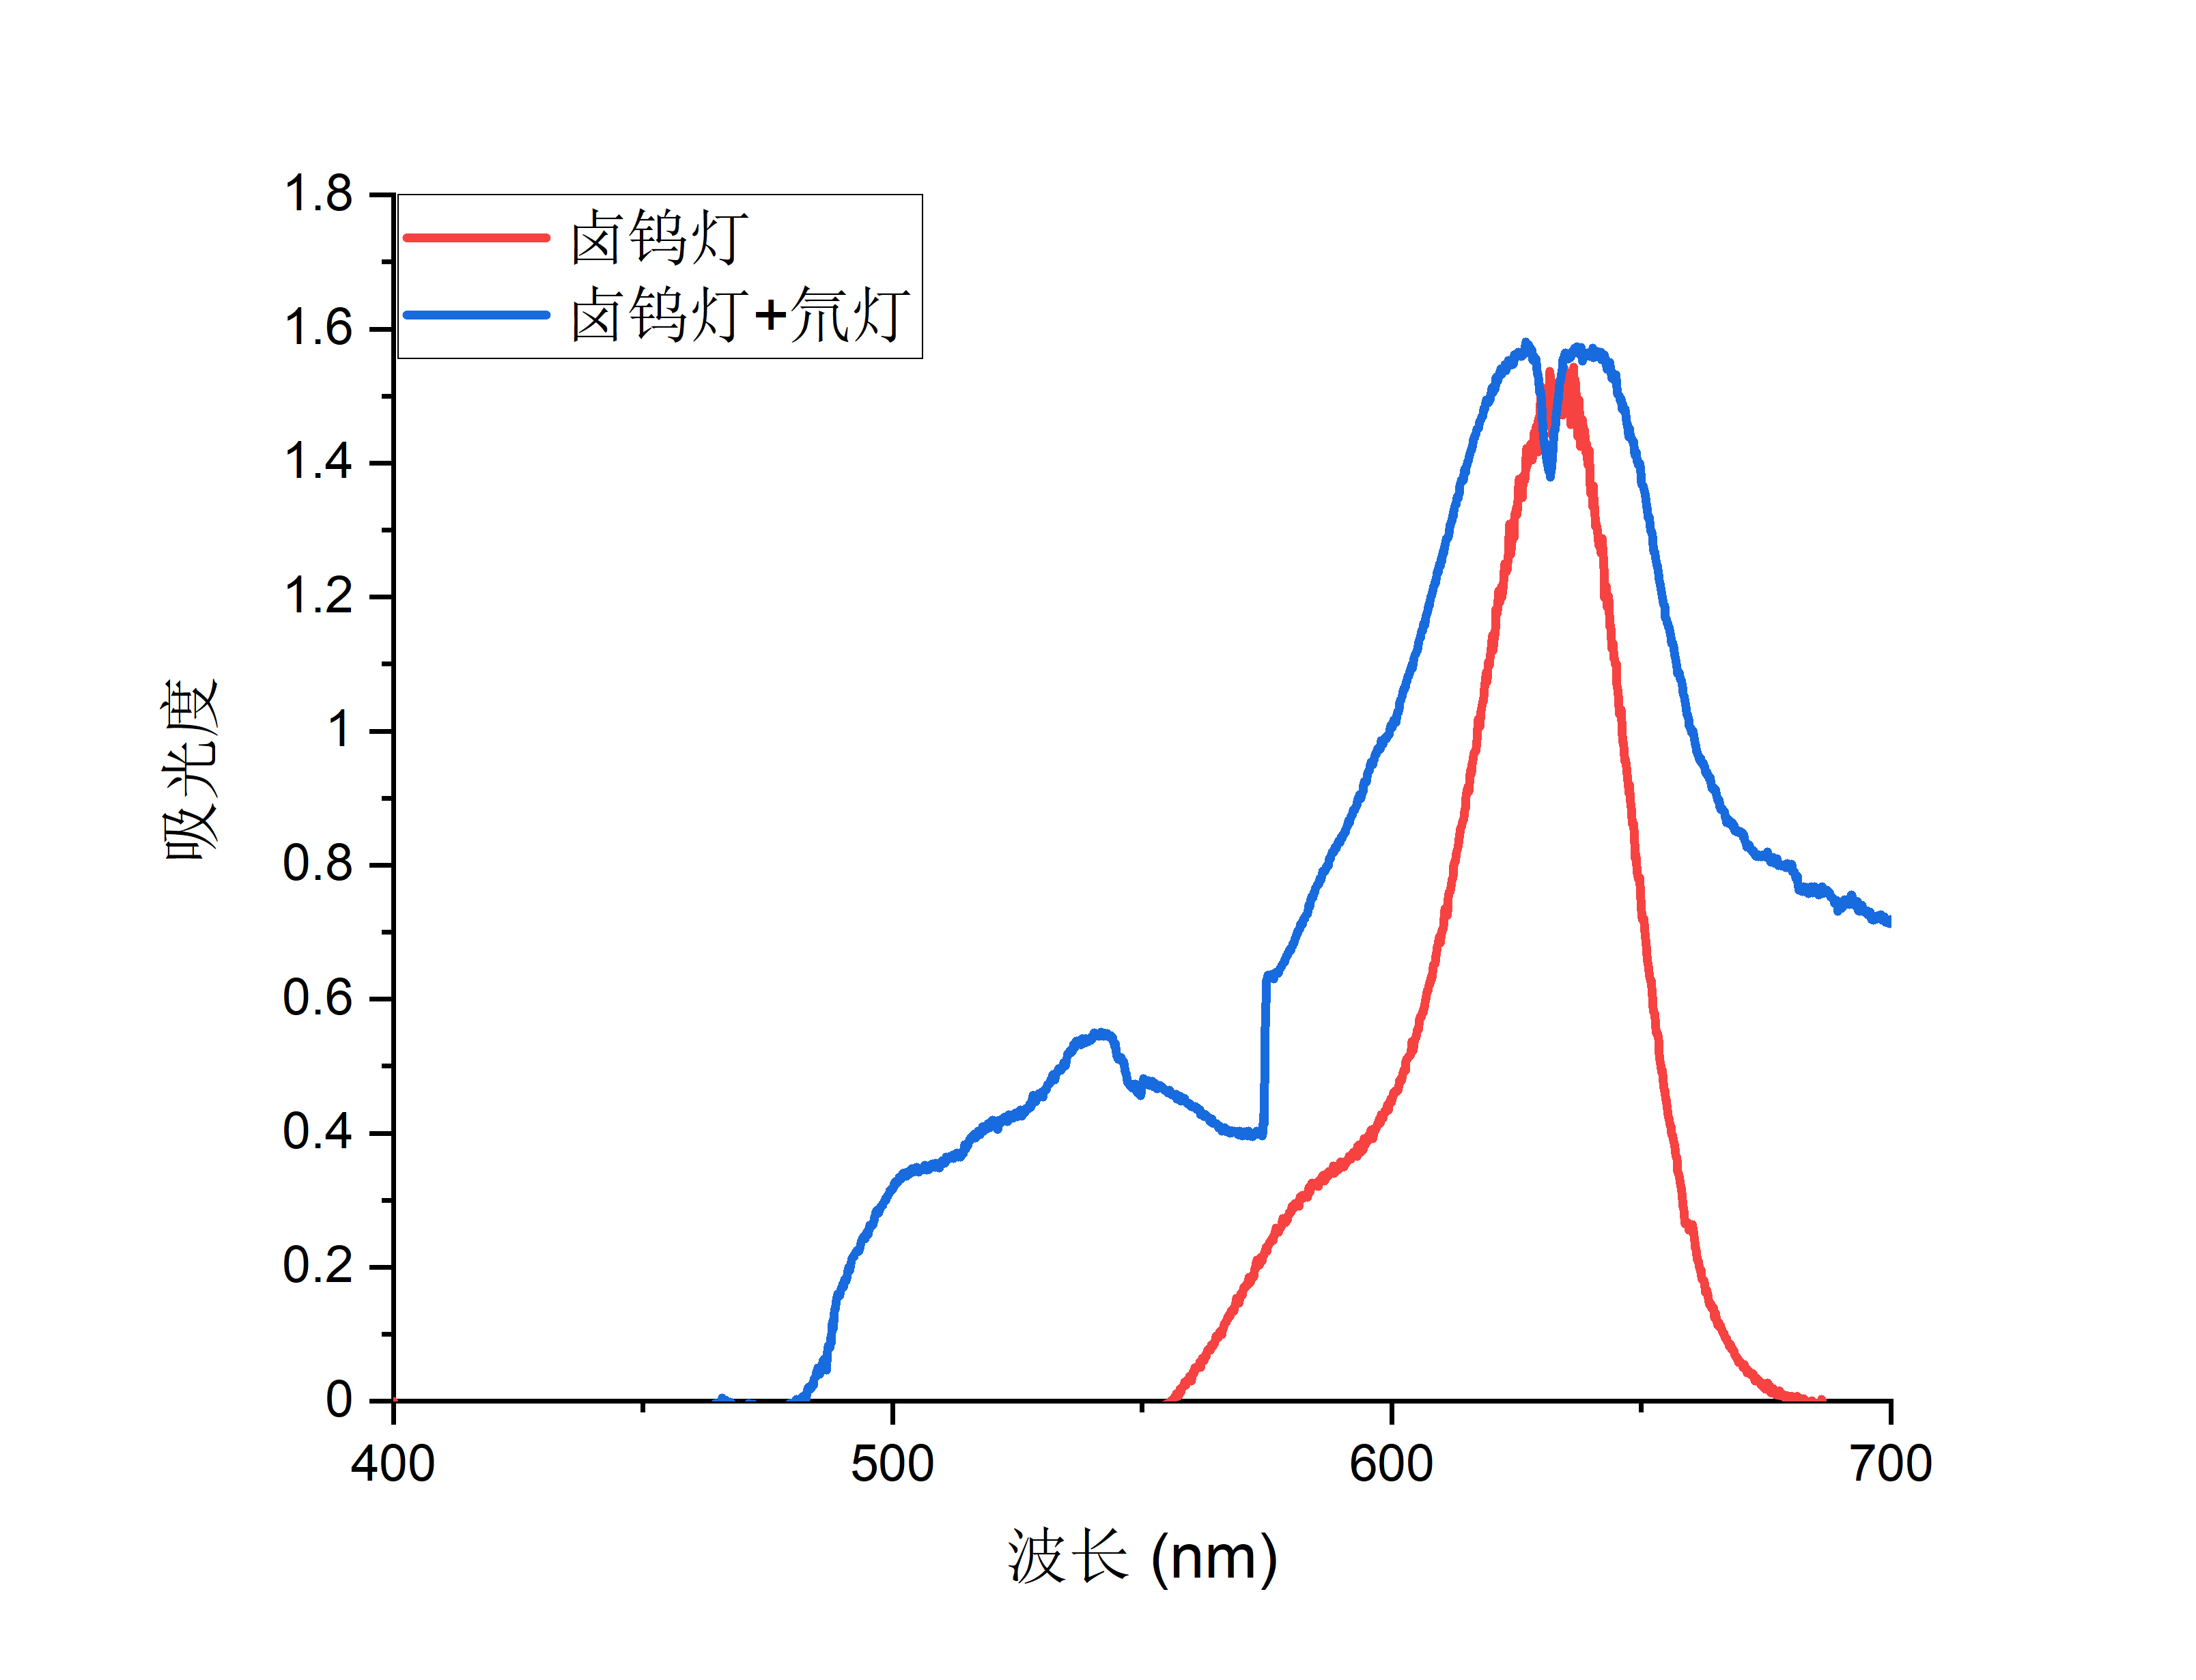
\includegraphics[width = .70\textwidth]{image/guangyuan.png}
    \caption{不同光源下 A3 分子吸收光谱}\label{25}
\end{figure}



从图中可以得到在两种光源下最大吸收波长几乎相同,但是卤钨灯与氘灯合用后光的亮度过高,导致峰的噪音很大。
应当适当调节狭缝大小以得到更好的结果。使用卤钨灯能够得到信噪比较低的结果,因此在接下来的测量中均使用卤钨灯作为光源进行实验。

\subsubsection{一维势阱的微扰模型}

在利用花青染料等分子进行一维势阱的验证中,我们看到 A 组分子可以较好地符合一维势阱模型,但仍有一些误差
,而 B 组分子与一维势阱模型的结论相差甚远。在 Utschbash 等人的工作中\cite{doi:10.1021/ed084p1840},
考虑到芳环对此类分子的的离域作用。使用了微扰理论对
简单的一维势箱进行了修正,对 A 组分子考虑使用简谐势作为微扰势,则对每一个能级的一阶微扰修正为
\begin{equation}
    E_{n}'=\int _{0}^{L}\psi ^{\ast}_n (x) V'(x) \psi_n (x) dx ,\ V'(x) = A\cos(\frac{2m\pi}{L} x)
\end{equation}

其中A为微扰势的强度,经过计算可以得到
\begin{equation}
    E_{n}'= \frac{An^2}{\pi} \frac{\cos(m\pi)\sin(m\pi)}{mn^2-m^3}
\end{equation}

在计算势箱长度时,引入偏移量 b 对芳环参与共轭进行了修正,我们利用已有的 A1 分子数据对其进行拟合得到下表 \ref{20} 的结果

\begin{table}[h]
    \centering
    \caption{微扰修正后的吸收波长}
    \label{20}
    \begin{tabular}{ccccc}
    \hline
    分子 & \multicolumn{1}{l}{势阱长度 / $\rm \mathring{A}$} & 微扰能量 / atomic units & 波长 / nm & 实验波长 / nm \\ \hline
    A1 & --                                   & --                  & --  & 428.53    \\
    A2 & 13.309                               & 0.0858              & 530.89  & 560.37    \\
    A3 & 15.803                               & 0.0719              & 633.35  & 637.35    \\
    A4 & 18.297                               & 0.0619              & 735.83  & 756.43    \\ \hline
    \end{tabular}
\end{table}

通过对比可以看出,这一修正对 A3 与 A4 拟合较好,但是对 A2 分子有较大的误差。文献中提到该方法对聚烯烃型双键也有较好的拟合效果
。但是由于B组分子的数量较少,B1 与 B2 在结构上的相似性不大,因此在此不进行计算。总之,本方法是一种对一维势箱模型的修正方法,具有较好的普遍性与准确性。



\subsubsection{理论计算方法探究}

在理论计算部分,由于设备的局限仅仅是用了半经验的方法对分子进行了模拟。接下来考虑在有充足计算资源的情况下应当如何计算两组分子的结构与紫外可见光谱图。

本次实验中的 A 组与 B 组分子均为大共轭分子,包含大量的离域 $\pi$ 电子。
对于这类分子,使用纯泛函和未极化的基组可能会出现较大的离域化误差和自相互作用误差,
运用这些方法进行激发态计算可能会产生不准确的结果。因此我们可以考虑使用 LC-$\omega$PBE, $\omega$B97X-D, CAM-B3LYP 等长短分程泛函
对这些分子进行计算。

基组上可以考虑使用一些极化基组,如 6-31g(d,p),若计算资源充足也可以考虑使用 cc-pVTZ 等较大的基组。最后,在计算中也要考虑溶剂化作用,
可以使用 SMD 隐式溶剂模型考虑体系的溶剂化。

使用以上方法可以较好地计算 A 组与 B 组分子,然而,最终的计算结果还将受到计算参数的选择、初始结构的准确性以及数值方法的影响。
因此,最终的计算方法也应当结合实际计算结果进行进一步的调整。





\subsection{结论}

在本次试验中,我们搭建了紫外可见光谱仪,测量了不同浓度下的 A 组与 B 组分子的紫外可见吸收光谱。
最终确定了合适的吸光度大小与光源,得到与文献报道相接近的结果。
结合实验的数据,我们通过一维势箱模型,修正后的一维势箱模型以及理论计算的方法对实验结果进行了验证
一维势箱理论模型可以较好描述 A 组分子,但是不能很好地拟合 B 组分子。我们使用修正后的一维势箱模型
也可以对 A 组分子给出较好的结果。再通过 Gaussian 与 Multiwfn 等计算软件,对这些分子用 AM1 方法进行半经验的理论计算。
囿于计算资源的局限性,A 组分子的模拟结果较差,B 组分子虽然存在一定的波长差异,但是给出了相对准确的波形。


\nocite{*}
\bibliography{reference}


\end{document}


%
%\section{实验目的}
%
%\begin{enumerate} %有序列表
%    \item 了解量子力学一维势阱模型
%    \item 了解紫外可见光谱仪的原理和构成
%    \item  学习紫外可见光谱仪的搭建和调试
%    \item 测定一些共轭分子的紫外可见光谱
%    \item 验证量子力学一维势阱公式
%\end{enumerate}
%
%\section{实验原理}
%
%\subsection{一维势阱中的能量量子化}
%
%    由薛定谔方程
%    
%    \begin{equation*}
%        \left(-\frac{\hbar^2}{2 m} \frac{\partial^2}{\partial x^2}+V(x)\right) \psi=E \psi
%    \end{equation*}
%    
%    可得
%    
%    \begin{equation*}
%        E=\frac{n^2h^2}{8mL^2}
%    \end{equation*}
%    
%    其中,n为量子态,m为粒子质量,L为势阱长度,h为普朗克常数。\\
%    \quad在线性共轭分子中,π轨道电子可以近似认为是在一维势箱中的粒子。
%
%\subsection{紫外可见光谱}
%    紫外可见光谱可以测定电子的跃迁,其中波长与能级差的关系为
%    
%    \begin{equation*}
%        \Delta E=\frac{hc}{\lambda }
%    \end{equation*}
%
%    对于电子与吸收量之间的关系,一般使用Lambert-Beer定律计算
%
%    \begin{equation*}
%        A=lg\frac{I_0}{I}=\varepsilon cb
%    \end{equation*}
%
%\section{实验原理}
%
%
%\begin{figure}[htbp]
%    \begin{minipage}{0.49\textwidth}
%        \centering
%        %\subfigure{
%        %    \centering
%        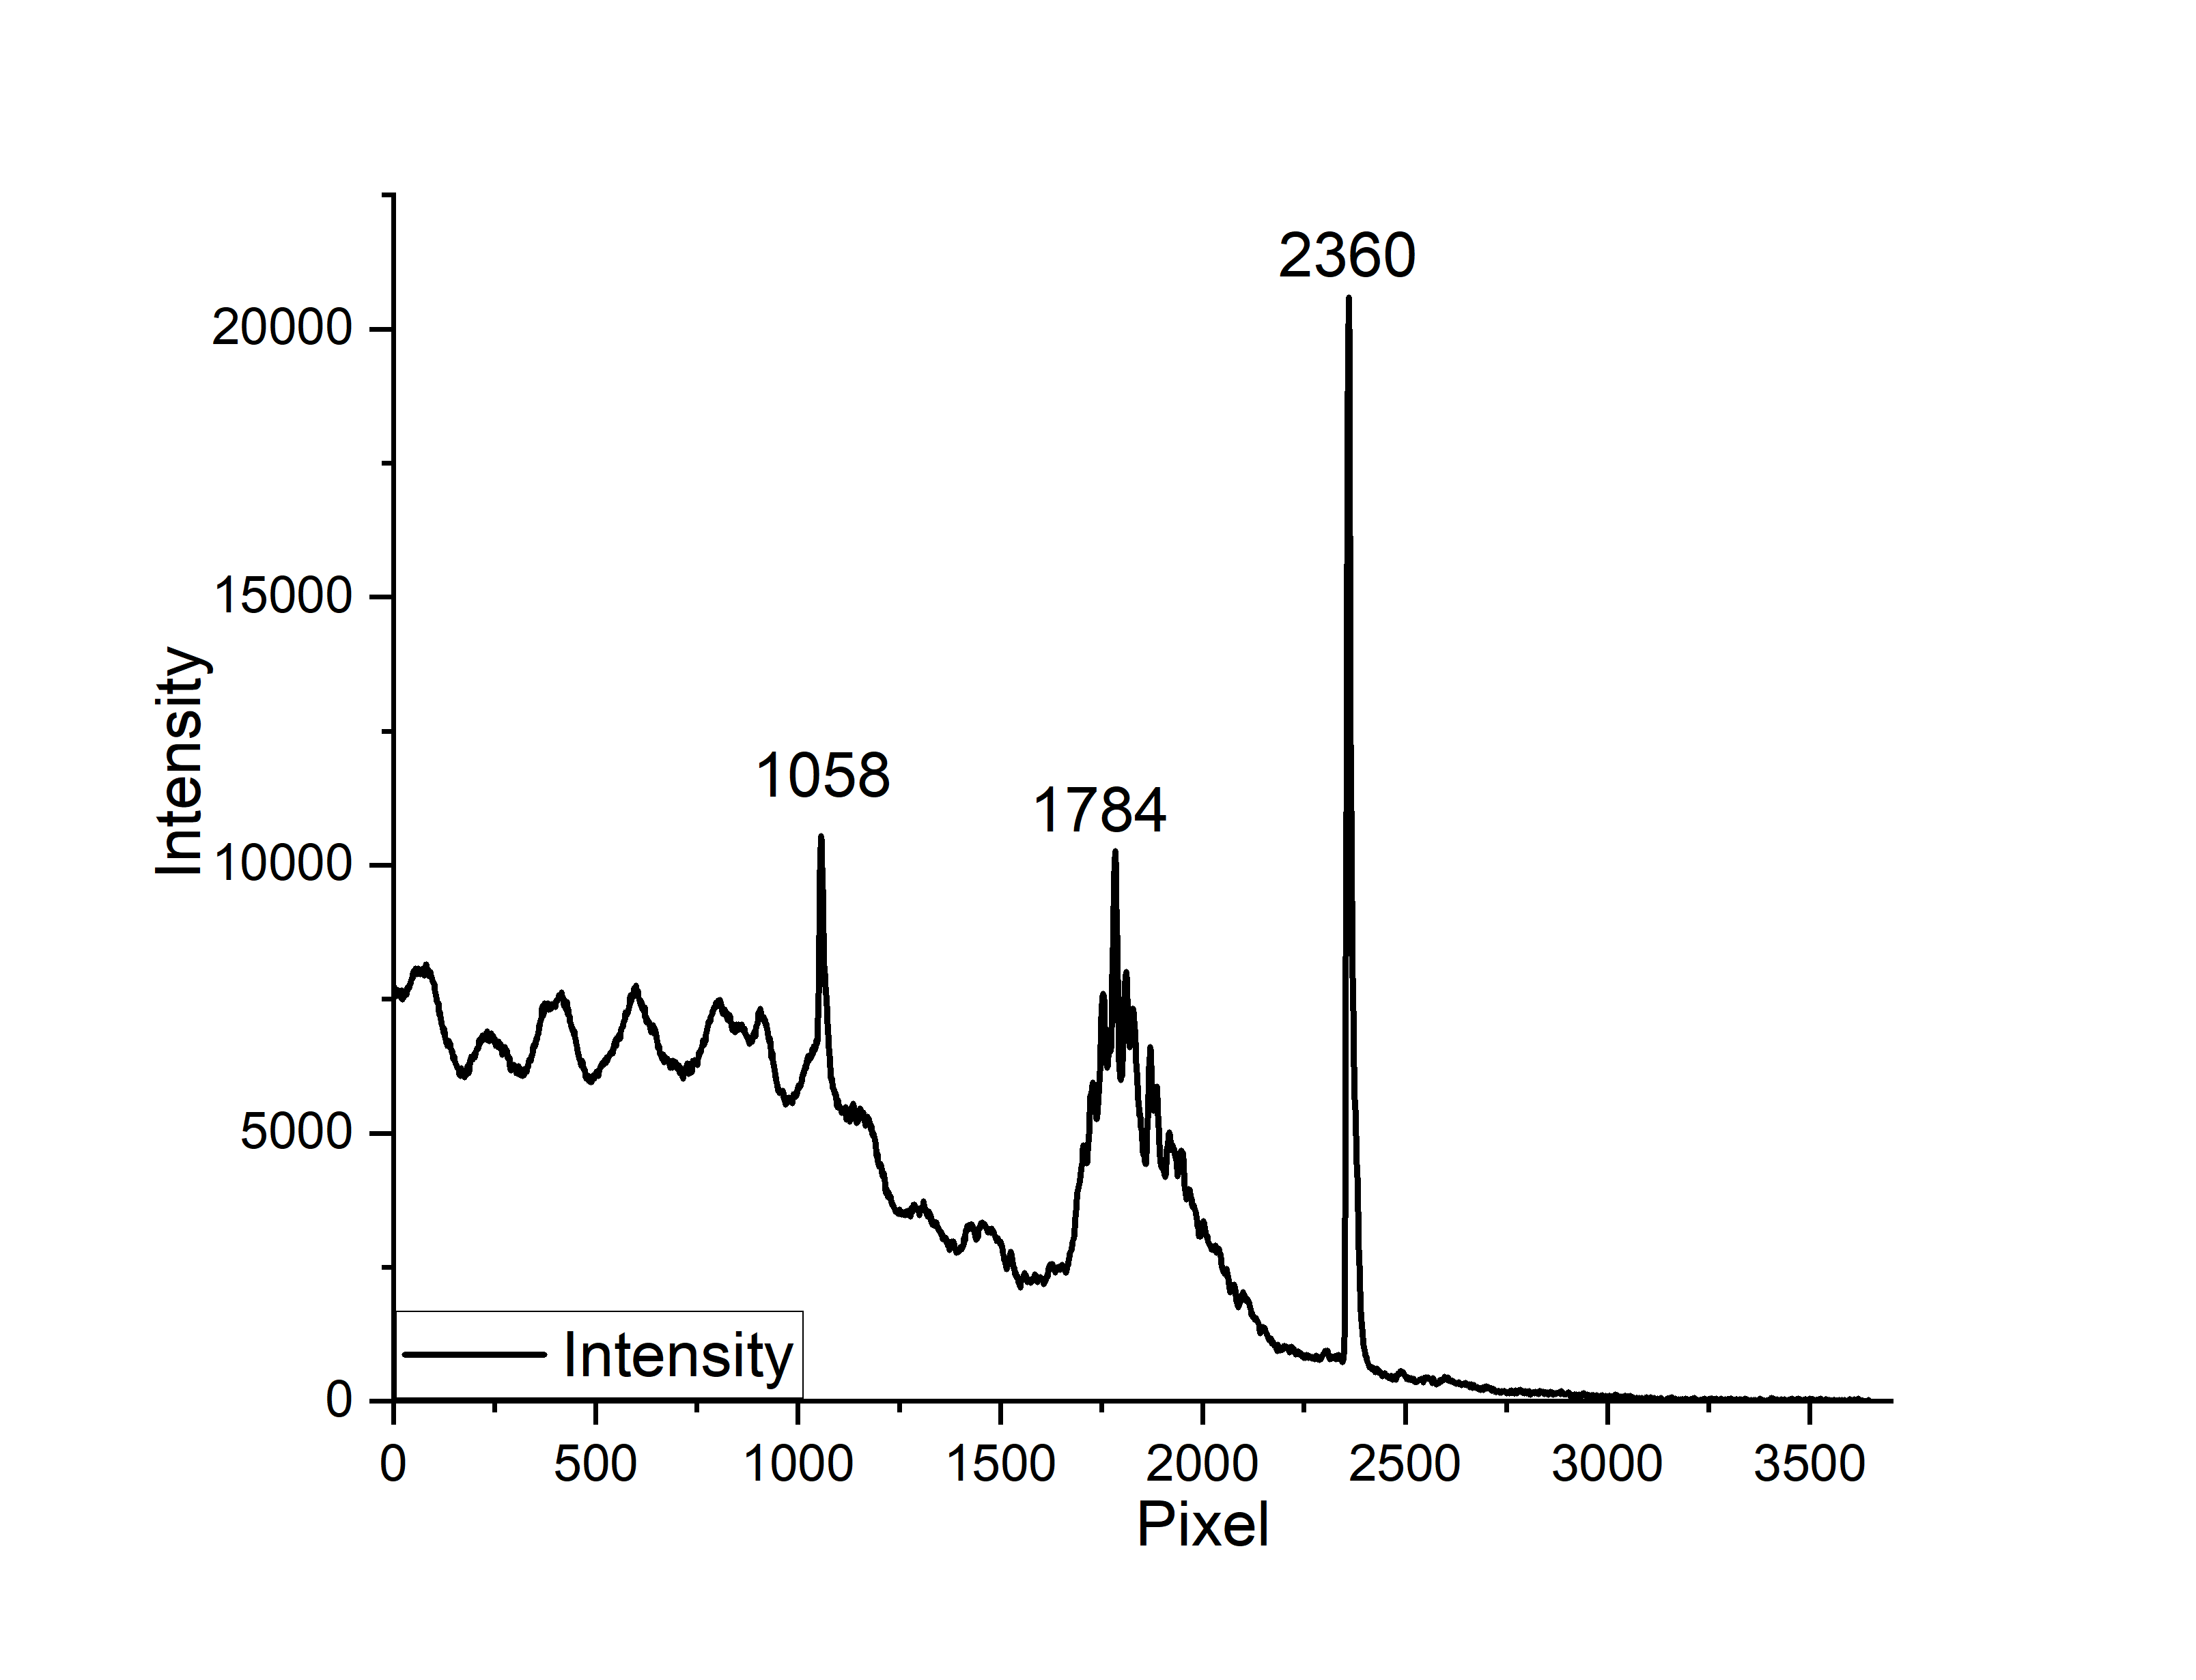
\includegraphics[height = 2.5in,width = 3.2in]{image/biaoding.png}
%        \caption{氘灯标定下的光强-像素图}\label{5--}
%    \end{minipage}
%    %}
%    \centering
%    %\subfigure{
%    \begin{minipage}{0.49\textwidth}
%        \centering
%        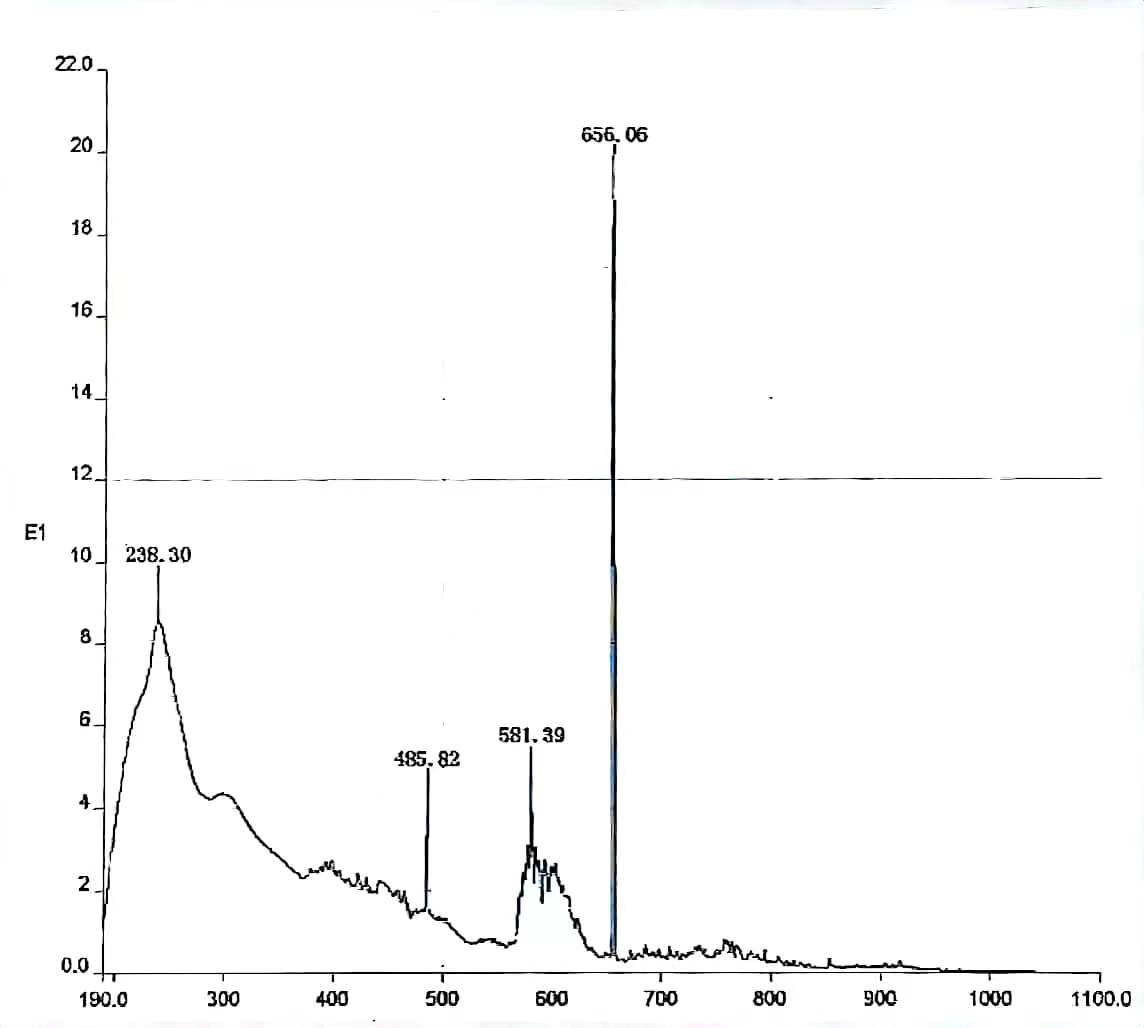
\includegraphics[height = 2.5in,width = 3in]{image/standard.jpg}
%        \caption{氘灯的标准光强-像素图}\label{5-}
%    \end{minipage}
%    %}
%    \centering
%    %\caption{左:氘灯标定下的光强-像素图\quad右:氘灯的标准光强-像素图}\label{5}
%\end{figure}